\documentclass[journal]{IEEEtran}
\usepackage{amsmath}
\usepackage{graphicx}
\newcommand{\resultfigure}[1]{%
  \IfFileExists{#1}{\includegraphics[width=\columnwidth]{#1}}{%
    \fbox{\parbox[c][0.20\textheight][c]{0.96\columnwidth}{\centering Result figure pending upload.}}%
  }%
}
\usepackage{tikz}
\usetikzlibrary{arrows.meta,positioning,fit,calc,backgrounds,fadings}

\ifCLASSINFOpdf

\else

\fi

\hyphenation{op-tical net-works semi-conduc-tor}


\begin{document}

\title{Reinforcement Twinning of MAV flying over an Obstacle in Ground Effect}

\author{Alessandro Grava and Miguel A. Mendez%
\thanks{A. Grava and M. A. Mendez are with the Department of Control Engineering and System Analysis (SAAS), Universit\'e libre de Bruxelles, Avenue Franklin Roosevelt 50, CP 165/55, 1050 Brussels, Belgium, and also with the von Karman Institute for Fluid Dynamics, Waterloosesteenweg 72, 1640 Sint-Genesius-Rode, Belgium.}%
\thanks{M. A. Mendez is also with the Department of Aerospace Engineering, Universidad Carlos III de Madrid, Avenida de la Universidad 30, 28911 Legan\'es, Madrid, Spain.}}

\markboth{}{}
\maketitle

\begin{abstract}This work presents an implementation of Reinforcement Twinning (RT) applied to a micro aerial vehicle operating in ground effect. The framework couples a Crazyflie 2.1+ as physical environment with its Digital Twin (DT) whose aerodynamic correction to account for ground effect is progressively identified from flight data. During a first information phase, the DT and the remaining uncertainty on the corrective parameters guide the design of information-oriented policies to be deployed on the physical environment. During a subsequent performance phase, model-based optimization first provides a safe and computationally efficient policy, while a reward-transfer surrogate combines DT and physical environment rewards to guide data-efficient policy refinement despite residual model error. The resulting policy is implemented as a lightweight spatial reference correction that retains the standard onboard feedback controller. Experiments over a finite obstacle show that the proposed workflow constrains the dominant ground-effect response over the tested clearance range and improves trajectory tracking with a limited number of physical interactions. A proof-of-concept extension to different operating conditions further illustrates how the same workflow can adapt a transferred correction when its performance changes away from the nominal condition. These results support the use of an adaptive DT for model learning and control improvement without exhaustive model-free exploration in the physical environment.\end{abstract}

\begin{IEEEkeywords}Reinforcement Twinning, digital twins, micro aerial vehicles, ground effect, system identification, predictive control, Bayesian optimization.\end{IEEEkeywords}

\IEEEpeerreviewmaketitle

\section{Introduction}
\label{Introduction}

\IEEEPARstart{I}{nterest} in unmanned aerial vehicles (UAVs), also commonly known as drones, has grown rapidly over the past years. Their use now extends beyond recreational flight, providing support in a wide range of complex operations. Active research is carried out in various civil applications~\cite{Shakhatreh2019}, with documented examples that go beyond simple demonstrators, including support during emergency operations~\cite{Ray2022}, aerial assessment of damaged buildings~\cite{Surmann2024}, and bridge inspection combining automated damage screening with human assessment~\cite{Bartczak2025}.
This growing interest is accompanied by substantial expectations for the sector. According to the European Commission, the European commercial airborne-drone market is forecast to reach approximately EUR~14.5 billion by 2030 and potentially exceed EUR~50 billion by 2033~\cite{EuropeanCommission2026}. At the global level, IMARC Group forecasts the commercial drone market to grow from USD~38.2 billion in 2025 to USD~189.9 billion by 2034~\cite{IMARC2026}.

The appeal of UAVs mainly stems from their ability to perform tasks without a pilot on board, either under remote control or autonomously. This feature, together with their reduced dimensions and capacity to carry small cameras and other sensors, permits observations and measurements to be acquired remotely from locations that are difficult to access using ground-based equipment or hazardous for human operators~\cite{ZhangInspection2024}. 
For missions in confined spaces, such as indoor environments, Micro Aerial Vehicles (MAVs) are particularly attractive due to their even smaller dimensions compared with typical commercial multirotors. In the size-based classification reviewed by Elmeseiry et al.~\cite{Elmeseiry2021}, MAVs have maximum dimensions between 7.5 and 15~cm. This feature permits access to narrow passages and cluttered environments~\cite{Floreano2015,ZhouSwarm2022}, facilitating the inspection of machinery, industrial installations, and damaged structures in which the available space restricts both human access and the use of larger aerial vehicles. 
Indoor flight places further demands on the vehicle and its control performance. Satellite positioning is generally unavailable, the surroundings may be only partially known, and sensing, actuation, and computation must be accommodated on a small platform with limited computational capacity. In cluttered environments, the available clearance might also leave little room for tracking errors. A trajectory that is geometrically collision-free may consequently be difficult to execute reliably. 
The flow induced by the MAV rotors can interact with floors, walls, ceilings, and other obstacles, altering the generated forces and moments~\cite{Carter2021}. These interactions can produce significant trajectory-tracking errors during flight~\cite{NeuralLander2019}, potentially compromising obstacle clearance and increasing the risk of collision in cluttered environments.

A reliable controller for indoor flight therefore requires control strategies that can predict aerodynamic interactions and compensate for their effects before substantial trajectory deviations develop. Their effectiveness depends on the accuracy of the physics-based model that describes the interaction, which can be augmented with experimental data, as demonstrated in hybrid control approaches for similar applications~\cite{LeeSparseGE2025,NeuralFly2022}. This introduces two connected questions: which experiments should be performed to improve the model, and how their results can be used to improve control performance when the model remains imperfect. Reinforcement Twinning (RT)~\cite{SchenaRT2023,Mendez2026} addresses these questions by coupling the physical system with an active, physics-based digital twin (DT). The DT is used to design missions optimized either to improve the accuracy of its physical model or to find control policies that improve performance on the physical system. The resulting experimental observations are used to update the model and learn the remaining discrepancies between virtual and measured performance. These discrepancies then guide further policy optimization, allowing improvements on the physical system beyond those obtained by optimizing the DT predictions alone.
In the present implementation, identification and policy optimization are performed offline, and the resulting references are supplied to the existing onboard feedback controller. This separates the computational demands of policy optimization from onboard trajectory execution, making the implementation particularly suitable for MAVs with limited computational resources.

The application of RT to a MAV flyingclose to an obstacle builds on both the physical understanding of rotor-surface interactions and the methods available to improve control through experimental data. The following subsections review these two aspects before discussing how they are brought together within RT.

\subsection{Aerodynamic interactions of MAVs with obstacles} 
Aerodynamic interactions between MAVs and nearby obstacles can often be divided into three elementary configurations: ground, wall, and ceiling effects. These configurations are mainly distinguished by the orientation of the surface relative to the rotor plane. Several interactions may occur simultaneously in confined environments, for instance during flight through a pipe or a narrow channel, where the vehicle is surrounded by multiple boundaries. Such scenarios can involve recirculation of the rotor wake and strong, unsteady force and moment disturbances, substantially complicating control and task success~\cite{Bauersfeld2026}.

Wall and ceiling effects have received increasing attention in recent years, with studies spanning small-scale rotors and quadcopters~\cite{Franzetti2024,Cai2024}, including MAVs as well~\cite{Carter2021}. Near a ceiling, the modified rotor inflow can increase the thrust generated at a given rotor speed, producing an attraction towards the surface. This response can be destabilizing because an upward displacement brings the vehicle closer to the ceiling, increasing the related effect until collision if not contrasted~\cite{Carter2021}. Ceiling-effect behavior also depends on forward speed and rotor inclination, as examined by Cai and Gunasekaran~\cite{Cai2024}.
Near a wall, unequal aerodynamic loading of the rotors can produce lateral forces and rolling or pitching moments toward the wall itself. The resulting attitude disturbances can be important even when the change in total thrust remains modest~\cite{Carter2021,Franzetti2024}, potentially leading again to collision. 
Both wall and ceiling interactions can compromise flight stability, with the strongest effects generally occurring at short surface clearances. For the Crazyflie 2.0 MAV investigated by Carter et al.~\cite{Carter2021}, significant ceiling-induced lift changes occurred at distances below approximately one rotor radius ($R=23$~mm), while wall-induced changes in total lift exceeded 2\% only at clearances of a few millimetres.

In contrast, ground effect (GE) has been largely investigated in rotorcraft aerodynamics since the last century, including the classical analysis of Cheeseman and Bennett~\cite{CheesemanBennett1955}. For a rotor hovering above a horizontal surface, the downward wake impinges on the boundary and is redirected laterally. The associated pressure field modifies the inflow through the rotor disk, reducing the induced velocity and increasing the effective angle of attack of the blades. At a given rotational speed, a higher thrust can consequently be generated than in out-of-ground-effect (OGE) conditions. This thrust augmentation has subsequently been characterized in smaller rotorcraft. For a Crazyflie~2.0, Carter et al.~\cite{Carter2021} reported significant ground-induced lift changes at rotor-plane clearances below 4$R$. The aerodynamic influence therefore extended beyond the very short clearances at which the strongest ceiling and wall effects were observed on the same vehicle.
The application of isolated-rotor models to multirotors has required modifications to account for interactions among neighboring rotor wakes and the vehicle body. Sanchez-Cuevas et al.~\cite{SanchezCuevas2017} incorporated these contributions into a multirotor GE model, including the additional thrust associated with the fountain flow generated between the rotors and the underlying surface.
The investigation was extended to forward flight by Kan et al.~\cite{Kan2019}, using an AscTec Hummingbird to develop their models and a Crazyflie~2.0 to evaluate their predictions on a smaller vehicle. The Crazyflie experiments covered normalized forward velocities \(0 \leq v_\infty/v_h \leq 0.48\) and rotor-to-ground clearances up to \(5R\), where \(v_h\) denotes the induced velocity of a single rotor in hover. In their analysis of the Hummingbird data, GE depended more strongly on clearance than on forward velocity in the low-to-medium-speed regime, defined as $v_x/v_h\leq1.2$, where $v_h$ is the ideal induced velocity in hover. Velocity dependence became more pronounced at higher speeds, for which separate model expressions were introduced. The same qualitative trend was confirmed for the Crazyflie within the tested velocity range, with GE depending more strongly on surface clearance than on forward velocity.
The thrust augmentation induced by GE tends to displace the vehicle away from the underlying surface, increasing the local clearance. This differs from ceiling effect, which can attract the vehicle towards the overhead boundary. In a cluttered environment, however, every deviation form the desired trajectory may reduce clearance to a following obstacle along the flight path. GE can therefore compromise safe trajectory tracking despite displacing the vehicle away from the surface that generates it. Its influence at comparatively large clearances makes it particularly important to account for in cluttered environments.

Considerations made above are based on static or quasi-steady operating conditions. The development and decay of the interaction during transitions into and out of GE are therefore not explicitly represented. Sanchez-Cuevas et al.~\cite{SanchezCuevas2017} considered obstacle-crossing scenarios by accounting for the different thrust augmentation experienced by individual rotors under partial GE. However, the correction remains determined by the instantaneous rotor-surface configuration, without introducing a separate evolution equation for the aerodynamic response.
The temporal evolution of the flow can be represented through dynamic inflow models. Gennaretti et al.~\cite{Gennaretti2017} developed a finite-state, linear time-invariant model of rotor wake inflow in GE, identified from the responses of a high-fidelity aerodynamic solver to rotor kinematic perturbations. The resulting state equations reproduce the evolution of the induced flow following changes in rotor commands. Pasquali et al.~\cite{Pasquali2023} subsequently identified state-space inflow models from free-wake simulations, relating the inflow coefficients to aerodynamic hub loads and rotor-ground conditions. The models were validated against the nonlinear free-wake solver, including fixed-ground configurations. These formulations retain aerodynamic states whose evolution represents wake dynamics beyond a static thrust correction. The model accuracy is then improved under transient conditions, such as crossing a finite obstacles, but this comes at the cost of additional model complexity.

\subsection{From Model-based Control to Reinforcement Twinning}
The aerodynamic interactions described above can cause substantial deviations from an otherwise safe trajectory, potentially compromising obstacle clearance in cluttered environments. Compensation through the onboard feedback controller may be insufficient, particularly when disturbances develop rapidly and corrective action is taken only after a tracking error has appeared~\cite{Quan2017}. Model-based prediction can support anticipatory compensation, but its effectiveness depends on an accurate representation of the relevant physics~\cite{Borrelli2017}. As discussed above, aerodynamic models may involve uncertain parameters or omit interactions and transient effects that influence the vehicle response~\cite{YangGE2025,HeDynamicGE2024}. For approaches requiring online optimization, such as model predictive control~\cite{MPCReview2021}, sufficient onboard computational resources are also required. This requirement can become restrictive for MAVs, especially when greater model complexity is introduced to improve prediction accuracy. 

Hybrid approaches combining physical models with information learned from experimental data offer a way to improve prediction and control while retaining a computationally manageable representation of the system. 
In such approaches, the available physical model can be improved through experimental data, identifying or correcting the effects that are insufficiently represented. The learning problem can thus be focused on the uncertain contributions to the vehicle response. Adaptive and neural methods for GE compensation were investigated experimentally by Xu et al.~\cite{XuGE2022}, with smoother take-off and landing than with a conventional PID controller. In the approach of Lee et al.~\cite{LeeSparseGE2025}, a sparse online Gaussian process (GP) model was coupled to a robust dynamic-inversion controller, improving forward-flight GE compensation and tracking performance in simulation relative to the controllers considered for comparison. A limited set of data was retained to contain the computational burden. In Neural Lander, learned aerodynamic corrections reduced the reported vertical tracking error during a cross-table maneuver from 15.3 to 2.7~cm relative to a baseline nonlinear tracking controller~\cite{NeuralLander2019}. Learned interaction forces also improved close-proximity flight tracking in Neural-Swarm2~\cite{NeuralSwarm2022}. Beyond surface effects, an aerodynamic representation learned offline was adapted online through a low-dimensional set of coefficients in Neural-Fly~\cite{NeuralFly2022}, reducing the mean position tracking error by 66\% relative to a nonlinear tracking controller across the tested wind conditions. These results demonstrate tracking improvements from learned aerodynamic corrections, while the sparse representation used by Lee et al. and the limited online adaptation in Neural-Fly address the associated computational demands.

The improved model can then be used to search for a control policy before additional physical experiments are performed. Following identification from flight measurements, the response to candidate policies is predicted in simulation and used for policy optimization. Physical experience thus supports policy improvement through the updated model, allowing multiple candidates to be assessed virtually between successive physical evaluations. More generally, this principle is central to model-based reinforcement learning, where a dynamics model can be learned from experience without requiring a predefined physical description. In the Dyna architecture, a model updated from physical experience is used to generate simulated experience for planning~\cite{Sutton1991}. In PILCO, a probabilistic dynamics model is learned from physical observations and used for policy search while accounting for prediction uncertainty~\cite{Deisenroth2011}. Virtual policy search can therefore reduce the experimental burden, although a policy optimized using the model may exploit inaccurate predictions and perform less favorably on the physical system.
 
The discrepancy between predicted and measured performance can also be addressed at the policy level. Once a useful control solution has been obtained, further improvement can be guided by physical evaluations without requiring a more accurate dynamics model. In this case, learning is directed towards the control decisions responsible for performance, while the available model or controller provides a starting point. Neural dynamics and model-based control were used to initialize a policy before model-free fine-tuning by Nagabandi et al.~\cite{Nagabandi2018}. A conventional controller can also be retained and supplemented with a learned correction, as investigated in residual reinforcement learning by Johannink et al.~\cite{Johannink2019}. An application to close-proximity quadcopter flight is provided by ProxFly~\cite{ProxFly2025}. In these approaches, experimental feedback is used to address the performance limitations of an available control solution, even when the underlying physical model remains incomplete.
 
The benefits of model correction and policy refinement depend on the quality of the physical experience available for learning. The conditions explored during an experiment determine which features of the dynamics can be identified and which policy improvements can be assessed. In adaptive control, measurements are used to update the model and adjust the controller, as in self-tuning regulators~\cite{Astrom1973}. However, successful regulation does not necessarily provide informative data: a MAV kept close to a nominal operating condition may scarcely excite the dynamics associated with uncertain parameters. Repeating the same mission can improve the estimates through repeated measurements while leaving some parameter combinations poorly distinguishable. In optimal experiment design, the inputs are therefore selected to make the measured response more informative about the parameters to be identified~\cite{Mehra1974,Goodwin1977,Hjalmarsson2005}. In dual control, information gathering is considered together with control performance: an action is evaluated through its immediate effect on the system and the knowledge it can provide for subsequent decisions~\cite{Feldbaum1960,Filatov2000,Mesbah2018}. Experiment selection thus becomes part of the learning process, with informative excitation and control performance providing complementary objectives.

When the objective is to improve physical control performance, experiment selection must identify which candidate policy is most promising to evaluate next. The experimental cost of this search is particularly important for MAVs: complex policy corrections may require extensive data, while each flight entails effort and a risk of undesirable vehicle responses. When the policy can be modified through a small set of parameters, Bayesian optimization provides a way to direct this search using relatively few evaluations. A probabilistic surrogate of the measured performance is fitted, and an acquisition criterion such as Expected Improvement is used to select the next policy to be tested~\cite{Mockus1975,Jones1998}. Both the predicted performance and its uncertainty contribute to the selection, allowing promising policies and insufficiently explored regions to be investigated.

The performance surrogate can also be informed by model predictions, reducing its reliance on physical evaluations alone. Simulated assessments provide an initial indication of which policies may perform well, while physical measurements reveal the accuracy of that indication. Simulation-informed Bayesian optimization was investigated for bipedal robots by Rai et al.~\cite{Rai2019}, including the consequences of disagreement between simulation and hardware. More recently, DT-guided Bayesian optimization has been developed for data-efficient controller tuning~\cite{Nobar2025}, and corrected DT predictions and physical measurements have been combined in a multi-fidelity formulation~\cite{Nobar2026}. These approaches are related to the broader use of calibrated computer models and discrepancy surrogates~\cite{Kennedy2001,Forrester2007}. A model can thus guide the experimental search while measured performance is used to learn the correction needed for its predictions to be useful on the physical system.

The identification and policy-search methods discussed above address two complementary needs: obtaining an informative description of the dynamics and improving control performance despite the errors that remain in that description. In Reinforcement Twinning (RT), both objectives are pursued through the coupling of a physical environment with an active, physics-based Digital Twin (DT)~\cite{SchenaRT2023,Mendez2026}. Physical observations are used to improve the DT, and subsequent experiments and control policies are designed within it to pursue further identification or performance improvement. This active role is consistent with the interpretation of digital twins as representations used to steer the systems they describe~\cite{Korenhof2021,Wagg2025}. RT shares with dual control the use of actuation to obtain information. Its information and performance objectives are organized through episode selection and model-assisted policy search, without requiring both objectives to be balanced within a single action-level optimization at every timestep~\cite{Mendez2026}. In earlier RT formulations, model-based and model-free learning were combined through policy switching and transfer, allowing the model to support initial control and physical experience to enable further policy improvement~\cite{SchenaRT2023,PolettiRT2025}.

The connection between experiment selection and policy improvement is made explicit in the twin-calibrated Bayesian formulation of Mendez et al.~\cite{Mendez2026}. Information-oriented episodes are designed using the current DT to improve its identification, while performance-oriented episodes are selected through a return transfer surrogate. In this surrogate, the virtual return supplies an affine-calibrated trend and a GP discrepancy represents the remaining dependence of the physical return on the policy. Here, the quantity corrected by the GP is the predicted return, whereas the learned aerodynamic corrections discussed earlier act on the dynamics model. Expected Improvement is then used to guide further physical evaluations. Learning the discrepancy at the level of performance allows policy improvement to continue even when the chosen physical model cannot reproduce every feature of the measured response. 

An experimentally assessed model-based policy provides a useful starting point for performance search. Local modifications can initially be evaluated within a restricted candidate domain, which can subsequently be expanded when further exploration is warranted. This strategy supports data efficiency and limits unrestricted physical exploration, although virtual screening alone cannot guarantee physical safety.

\subsection{Contribution of this work}
In the present work, RT is evaluated experimentally for altitude tracking of a Crazyflie~2.1+ flying over a finite horizontal obstacle at low clearance. The resulting GE disturbs the vehicle trajectory and provides a test case for anticipatory control under imperfect aerodynamic modeling. A six-degree-of-freedom DT based on Richardson and Pretorius~\cite{Richardson2025} is augmented with a deliberately simple static GE model, whose coefficients are initially uncertain and whose formulation omits unsteady aerodynamic effects. The information phase is first conducted to identify these coefficients through informative flights. The identified model is then frozen and used to optimize a model-based reference trajectory. In the subsequent performance phase, the discrepancy between virtual and physical returns is learned to guide further trajectory refinement beyond the model-based solution. Throughout the campaign, the existing onboard PID controller is retained, and the optimized position references are supplied to it. Identification and policy optimization are performed offline, keeping these computations off the vehicle. Policy transfer and further refinement are also assessed at different desired clearances and forward velocities. The experimental contribution is to assess how much tracking improvement can be obtained from a deliberately simple physical model through parameter identification, and how the remaining performance limitations can subsequently be addressed through learned return transfer.
 
The remainder of the paper is organized as follows. Section~\ref{sec:methodology} presents the RT framework. The physical and digital environments and the experimental workflow are described in Section~\ref{sec:setup}. The results are presented and discussed in Section~\ref{sec:results}, and the conclusions are drawn in Section~\ref{sec:conclusion}.

\section{Reinforcement Twinning Methodology}
\label{sec:methodology}
\label{sec:rt-framework}

Reinforcement Twinning (RT) couples a physical environment (EXP) with an active, physics-based Digital Twin (DT)~\cite{SchenaRT2023,Mendez2026}. The two environments evolve side by side and pursue complementary objectives. The EXP has a performance objective, achieved through the optimization of control policy parameters, whereas the DT must improve its physical model to predict the response of the EXP and propose improved control policies. Experience from the EXP is therefore used both as evidence to update the DT and as feedback on the policies designed with that DT. In turn, the DT adapts from these observations and proposes the next mission to be deployed on the EXP from which new observations are generated. This exchange allows model identification and performance improvement to support each other, while of the exploration and optimization takes place virtually before a selected policy is experimentally deployed, supporting safer and more efficient framework.

\subsection{Environments, observations and objectives}
The EXP and the DT are denoted by a filled circle $(\bullet)$ and an empty circle $(\circ)$, respectively, following the notation of Mendez et al.~\cite{Mendez2026}. During an episode $n$ carried out on the EXP, its state at the timestep $k$ is represented by $\mathbf s_{\bullet,k}^{(n)}$. Its evolution to the following timestep is described by
\begin{equation}
 \mathbf s_{\bullet,k+1}^{(n)}
 =\mathbf F_\bullet\!\left(\mathbf s_{\bullet,k}^{(n)},
 \mathbf a_{\bullet,k}^{(n)},\mathbf z_k^{(n)}\right),
 \label{eq:rt-physical-state}
\end{equation}
where the unknown dynamics are represented by $\mathbf F_\bullet$, the applied actions by $\mathbf a_\bullet$, and the exogenous input by $\mathbf z$. The latter includes disturbances and other inputs that are not selected by the policy. For readability, the superscript $n$ is omitted below when referring to quantities within a single episode.

In general, $\mathbf s_{\bullet}$ is only partially accessible through measurements. The available observation is denoted by $\mathbf o_{\bullet,k}$ and is expressed as
\begin{equation}
 \mathbf o_{\bullet,k}
 =\mathbf h(\mathbf s_{\bullet,k},\mathbf a_{\bullet,k-1})
 +\boldsymbol{\varepsilon}_{\bullet,k},
 \label{eq:rt-physical-observation}
\end{equation}
where the measured quantities are selected through $\mathbf h$. Measurement error is represented by $\boldsymbol{\varepsilon}_{\bullet,k}$. The previous action is included to accommodate measurements associated with actuation, while keeping the observation available before the current action is selected.

The objective within the EXP is to improve control performance through the optimization of a policy $\pi_\bullet(\cdot\mid\boldsymbol{\theta}_\pi)$, where $\boldsymbol{\theta}_\pi$ are policy parameters selected to maximize the expected physical return $\mathcal R_\bullet$:
\begin{equation}
 \boldsymbol{\theta}_\pi^\star
 =\arg\max_{\boldsymbol{\theta}_\pi\in\Theta_\pi}
 \mathrm E[\mathcal R_\bullet(\boldsymbol{\theta}_\pi)],
 \label{eq:rt-physical-objective}
\end{equation}
where the admissible $\boldsymbol{\theta}_\pi$ domain is denoted by $\Theta_\pi$. The optimal parameters are denoted by $\boldsymbol{\theta}_\pi^\star$ and define the optimal policy $\pi_\bullet^\star=\pi_\bullet(\cdot\mid\boldsymbol{\theta}_\pi^\star)$. Performance is assessed through the physical return $\mathcal R_\bullet$, and the expectation is taken over variations in initial conditions, exogenous inputs, and measurement error.

The corresponding state in the DT is denoted by $\mathbf s_{\circ,k}$ and is propagated through
\begin{equation}
 \mathbf s_{\circ,k+1}
 =\mathbf F_\circ(\mathbf s_{\circ,k},\mathbf a_{\circ,k},
                 \widehat{\mathbf z}_k;\boldsymbol{\theta}_p^{(m)}),
 \label{eq:rt-digital-state}
\end{equation}
where the dynamics are approximated by $\mathbf F_\circ$ and the recorded or estimated exogenous input is denoted by $\widehat{\mathbf z}$. The uncertain or unknown model parameters of the DT are collected in $\boldsymbol{\theta}_p^{(m)}$, with $m$ indexing accepted model updates. This index is distinct from the episode index $n$, since $\boldsymbol{\theta}_p$ need not be updated after every episode. A fixed structure is retained for $\mathbf F_\circ$ and only $\boldsymbol{\theta}_p$ are updated to reach a closer agreement between the physical and virtual environments.

The predicted observation is obtained from the simulated state as
\begin{equation}
 \overline{\mathbf o}_{\circ,k}
 =\mathbf h(\mathbf s_{\circ,k},\mathbf a_{\circ,k-1};
            \boldsymbol{\theta}_p^{(m)}).
 \label{eq:rt-digital-observation}
\end{equation}
The overbar denotes a prediction without added measurement noise. This prediction is compared directly with $\mathbf o_\bullet$ during identification.

The objective of the DT is to improve its agreement with $\mathbf o_\bullet$ through the identification of $\boldsymbol{\theta}_p$. To support effective identification, dedicated policies $\pi_\iota(\cdot\mid\boldsymbol{\theta}_\iota)$ are designed, whose parameters $\boldsymbol{\theta}_\iota$ are selected to explore conditions informative about $\boldsymbol{\theta}_p$, instead of maximizing control performance through Eq.~\eqref{eq:rt-physical-objective}. The estimate of $\boldsymbol{\theta}_p$ is then updated from the accumulated physical records according to
\begin{equation}
\boldsymbol{\theta}_p^{(m+1)}
 =\arg\min_{\boldsymbol{\theta}_p\in\Theta_p}
 J_p(\boldsymbol{\theta}_p\mid\mathcal B_n).
 \label{eq:rt-model-objective}
\end{equation}
The admissible $\boldsymbol{\theta}_p$ domain is denoted by $\Theta_p$, and the discrepancy between recorded and replayed quantities is measured by the identification loss $J_p$. All available episode records are collected in the replay buffer $\mathcal B_n=\{\mathcal E^{(1)},\ldots,\mathcal E^{(n)}\}$. Each $\mathcal E^{(n)}$ contains the observations, deployed policy, actions, available exogenous inputs, operating conditions, and evaluated return. Through the choice of residuals and weights in $J_p$, the identification is directed towards the quantities relevant to the application. Any discrepancy left by the assumed structure of $\mathbf F_\circ$ must subsequently be accounted for during policy search.

\subsection{Policy representation and episode schedule}
The interaction between the two environments is mediated by control policies that are designed within the DT and subsequently deployed in the EXP. Policy design is therefore performed virtually: candidate episodes can be evaluated and optimized before the selected policy is transferred to the EXP. The resulting physical episode then provides the experimental evidence required by the learning process. Depending on the current objective, either an information-oriented or a performance-oriented policy is designed in the DT.

The information-oriented policy $\pi_{\iota}(\cdot\mid\boldsymbol{\theta}_{\iota})$, with $\boldsymbol{\theta}_{\iota}\in\Theta_{\iota}$, is designed to generate observations that are informative about $\boldsymbol{\theta}_{p}$. Conversely, the performance-oriented policy $\pi_{\bullet}(\cdot\mid\boldsymbol{\theta}_{\pi})$, with $\boldsymbol{\theta}_{\pi}\in\Theta_{\pi}$, is designed using the current DT to maximize the expected physical return $\mathcal R_\bullet$. The two policy families may have significantly different parameterizations because their classification reflects the objective used during policy design. In the general framework, data generated by either policy family can support both objectives. A performance-oriented policy may excite dynamics that improve the estimate of $\boldsymbol{\theta}_p$, and useful performance information may also be obtained from an information-oriented episode. In the campaign adopted here, the return transfer surrogate is calibrated using only performance-oriented policies; the purely information-oriented episodes are excluded from this calibration.

In the present work, both policy families are implemented by modifying the position reference $\mathbf{x}^{\ast}=[x_x^{\ast},x_y^{\ast},x_z^{\ast}]^{\mathsf T}$ supplied to a baseline feedback controller. According to the current objective, the reference is parameterized by $\boldsymbol{\theta}_{\iota}$ or $\boldsymbol{\theta}_{\pi}$ and optimized in the DT before deployment. The baseline feedback controller and its gains are retained to generate the actions during execution. For performance-oriented design, this commanded reference may differ from the nominal task trajectory: performance is always assessed against the unchanged nominal target. Before each episode, consistent initial conditions are established in both environments, including the internal state of the baseline feedback controller.

A binary episode schedule $e_n\in\{0,1\}$ determines which policy is designed and deployed during each episode $n$:
\begin{equation}
\pi_{\bullet}^{(n)}=
\begin{cases}
\pi_{\iota}\!\left(\cdot\mid\boldsymbol{\theta}_{\iota}^{(n)}\right),
& e_n=1,\quad \text{information-oriented},\\[2mm]
\pi_{\bullet}\!\left(\cdot\mid\boldsymbol{\theta}_{\pi}^{(n)}\right),
& e_n=0,\quad \text{performance-oriented}.
\end{cases}
\label{eq:rt-policy-schedule}
\end{equation}

In the general RT formulation of Mendez et al.~\cite{Mendez2026}, these two types of episode may be alternated during the campaign as the DT and policy evolve. For simplicity, a sequential schedule is adopted here: information-oriented missions are performed first until the adopted identification and convergence requirements are satisfied. The identified $\boldsymbol{\theta}_p$ are then kept fixed (\textit{frozen model}), and the campaign is continued with performance-oriented missions. An initial \emph{information phase} and a subsequent \emph{performance phase} are therefore distinguished and described below.

\subsection{Information phase} 
At each identification step, the observations $\mathbf o_\bullet$ stored in $\mathcal B_n$ are compared with the corresponding DT predictions $\overline{\mathbf o}_\circ$. Since the policies adopted here are specified through spatial position references, the same $\mathbf x^\ast$ supplied during each physical episode is replayed in the DT. Each replay is initialized from the reconstructed initial state of the corresponding physical episode, including the internal state of the baseline feedback controller. 

After every information episode, $\mathcal B_n$ is enlarged, and $\boldsymbol{\theta}_p$ can be updated by solving Eq.~\eqref{eq:rt-model-objective} before designing and deploying another episode. Identification may be performed after each episode or after a batch of episodes. The index $n$ counts physical episodes, whereas $m$ counts accepted model updates.
A differentiable DT, such as the one adopted here, allows the gradient of $J_p$ to be computed through the replay and used for parameter estimation. Other identification methods can also be used within the same workflow. 
Once the fit has converged numerically at the update $m$, candidate reference trajectories are generated and evaluated in the DT to determine which episode should be performed next. The selection is directed towards improving the identification of the $\boldsymbol{\theta}_p$ combinations that are least constrained by the available observations. For this purpose, the information collected through the completed episodes is quantified using the Fisher information matrix, as used in optimal experiment design~\cite{Mehra1974,Goodwin1977}. After each identification update, this matrix is evaluated again using the current $\boldsymbol{\theta}_p$. The expected cumulative information after an additional candidate episode is expressed as
\begin{equation}
 \mathbf F_{n+1}(\boldsymbol{\theta}_\iota)
 =\mathbf F_n+
 \mathbf S(\boldsymbol{\theta}_\iota)^{\mathsf T}
 \boldsymbol{\Sigma}_o^{-1}
 \mathbf S(\boldsymbol{\theta}_\iota).
 \label{eq:rt-fisher-update}
\end{equation}
where the contribution of the completed episodes is denoted by $\mathbf F_n$. The second term represents the information expected from the potential next candidate specified by $\boldsymbol{\theta}_\iota$. Its predicted observations are differentiated with respect to $\boldsymbol{\theta}_p$, and the resulting sensitivities are collected in the Jacobian $\mathbf S(\boldsymbol{\theta}_\iota)$. Here $\boldsymbol{\Sigma}_o$ denotes the noise covariance of the full observation vector stacked over the candidate episode, and its inverse is used to weight the sensitivities. The additive update assumes that observation errors from different episodes are independent; correlations within an episode can be represented in $\boldsymbol{\Sigma}_o$. A parameter change is therefore considered more distinguishable when a larger change in the observations is predicted relative to the measurement noise. Consistent parameter scaling and episode weighting are used across candidates. When noise statistics are approximated or structural error is present, the matrix is interpreted as a comparative information metric.

The eigenvectors of the Fisher information matrix define directions in parameter space, each corresponding to a combination of parameter variations. The information available along each direction is quantified by the corresponding eigenvalue. The smallest eigenvalue therefore identifies the least-informed direction. Under the E-optimal criterion, the next mission is selected to maximize this eigenvalue, improving the ability to distinguish parameter variations along that direction. Equivalently, the information cost $\mathcal J_{\mathrm{info}}$ is defined as its negative, and the next policy parameters are selected by minimizing this cost:
\begin{equation}
 \boldsymbol{\theta}_\iota^{(n+1)}
 =\arg\min_{\boldsymbol{\theta}_\iota\in\Theta_{\iota,\mathrm{safe}}}
 \underbrace{-\lambda_{\min}
 [\mathbf F_{n+1}(\boldsymbol{\theta}_\iota)]}
 _{\mathcal J_{\mathrm{info}}(\boldsymbol{\theta}_\iota)}.
 \label{eq:rt-e-optimal}
\end{equation} 
Through this criterion, new episodes are directed towards information that complements the existing dataset, including combinations of parameters whose individual effects are difficult to separate. The set $\Theta_{\iota,\mathrm{safe}}$ contains candidates that pass the prescribed virtual checks on states, actions, and references. These checks depend on the predictive validity of the DT and provide screening, not a guarantee of physical safety.

A separate novelty check can supplement $\mathcal J_{\mathrm{info}}$, allowing a candidate with slightly lower predicted information to be chosen when it produces a sufficiently different response from those already recorded. The admissible design domain can also be revised to concentrate new experiments where sensitivity or uncertainty indicates a need for further data. The preceding records remain in $\mathcal B_n$.

After deployment, $\mathcal E^{(n+1)}$ is appended to the existing dataset and identification is repeated from the previous estimate. The information phase is ended when only small changes in the converged $\boldsymbol{\theta}_p$ estimates are obtained after new episodes are added and the magnitude of the estimated parameter correlation no longer decreases appreciably. 

Once the information phase is completed, a first model-based policy $\pi_{\mathrm{MB}}$ is computed by optimizing the reference trajectory in the identified DT:
\begin{equation}
 \boldsymbol{\theta}_{\pi,\mathrm{MB}}
 =\arg\max_{\boldsymbol{\theta}_\pi\in\Theta_{\pi,\mathrm{safe}}}
 \mathcal R_\circ(\boldsymbol{\theta}_\pi;\boldsymbol{\theta}_p).
 \label{eq:rt-mb-optimum}
\end{equation}
The solution $\boldsymbol{\theta}_{\pi,\mathrm{MB}}$ defines $\pi_{\mathrm{MB}}=\pi_\bullet(\cdot\mid\boldsymbol{\theta}_{\pi,\mathrm{MB}})$. Task-specific regularization can be added to discourage excessive or abrupt reference changes. The resulting policy is then deployed in the EXP to assess the initial improvement over $\pi_{\mathrm{BL}}$ obtained through model identification and predictive reference optimization. This policy provides the starting point for the subsequent performance phase, in which the remaining discrepancy between the two environments is addressed. If \(\boldsymbol{\theta}_p\) is held fixed during the performance phase, the DT is considered \textit{frozen}, and \(\pi_{\mathrm{MB}}\) is retained as the reference policy around which further improvements are sought.

\subsection{Performance phase}
In the formulation adopted in this work, $\boldsymbol{\theta}_p$ is kept fixed after the information phase. The performance phase is then directed towards improving $\mathcal R_\bullet$ deriving from $\pi_{\mathrm{MB}}$ by accounting for the discrepancies that remain between the DT and the EXP. Closer agreement between predicted and measured responses is expected after identification, but identical behavior is generally not obtained when the same policy is deployed in the two environments. Differences may be left by an incomplete model structure, insufficient identification of some parameters, or phenomena that are too complex to be represented within the adopted approximation.

Consequently, a policy optimized in the DT may be assigned a higher $\mathcal R_\circ$ than the correspondent $\mathcal R_\bullet$ obtained experimentally. In this case, an apparently effective action is less successful when deployed in the EXP. Discrepancies of the opposite sign are also possible. In either case, the policy with the highest $\mathcal R_\circ$ might not provide the highest $\mathcal R_\bullet$. Further improvement is therefore sought by modeling the transfer from $\mathcal R_\circ$ to $\mathcal R_\bullet$ using a return transfer surrogate model. This model is then exploited to select policies that lead to improved performance on the EXP. 
Following Mendez et al.~\cite{Mendez2026}, the return transfer surrogate is expressed as
\begin{equation}
 \begin{aligned}
 \mathcal R_\bullet(\boldsymbol{\theta}_\pi;\mathbf c)
 &=b_{\circ,0}
  +b_{\circ,1}\mathcal R_\circ
    (\boldsymbol{\theta}_\pi;\mathbf c,\boldsymbol{\theta}_p)\\
 &\quad+\delta(\boldsymbol{\theta}_\pi,\mathbf c)+\varepsilon,
 \qquad \delta\sim\mathcal{GP}(0,k_\delta).
 \end{aligned}
 \label{eq:rt-surrogate}
\end{equation}
The overall relation between $\mathcal R_\circ$ and $\mathcal R_\bullet$ is represented by an affine trend, with intercept $b_{\circ,0}$ and slope $b_{\circ,1}$. The discrepancy that depends on the policy and is not captured by this affine trend is modeled by the Gaussian process $\delta$. The operating conditions are collected in $\mathbf c$, allowing their influence on the discrepancy to be included when episodes at several conditions are available. Similar corrections are associated with nearby policies and conditions through the covariance kernel $k_\delta$, while return-observation noise is represented by $\varepsilon$.

For the present formulation, the return is normalized relative to the return obtained with $\pi_{\mathrm{BL}}$ to express improvement on a common scale across operating conditions:
\begin{equation}
 \mathcal R_e(\pi;\mathbf c)
 =1-\frac{J_e(\pi;\mathbf c)}
          {J_e(\pi_{\mathrm{BL}};\mathbf c)},
 \qquad e\in\{\bullet,\circ\}.
 \label{eq:rt-normalized-reward}
\end{equation}
Here the performance task cost is denoted by $J_e$ and is evaluated against the nominal task target, independently of the commanded reference used by the policy. Both costs in the ratio are evaluated in the same environment at the same $\mathbf c$, with a positive baseline cost. A return of zero is therefore assigned to $\pi_{\mathrm{BL}}$, and positive values indicate a reduction in cost relative to that baseline, therefore an improved return. A value of one corresponds to zero cost, whereas negative values indicate deterioration. The normalization allows relative improvements to be compared across operating conditions; any dependence of the remaining discrepancy on $\mathbf c$ must still be learned from the available data.

To avoid the experimental cost of a fully model-free search, surrogate calibration is started from two available reference policies: $\pi_{\mathrm{BL}}$, for which the normalized return is zero in both environments, and $\pi_{\mathrm{MB}}$, for which an improvement is expected from the identified model and assessed through physical deployment. When a favorable $\mathcal R_\bullet$ is already obtained with $\pi_{\mathrm{MB}}$, further improvement can be sought through local reference modifications within an initially restricted domain around this policy. Selected intermediate and neighboring policies are evaluated in both environments, and $b_{\circ,0}$, $b_{\circ,1}$, and $\delta$ are estimated from the resulting paired returns.
The search domain can be expanded as evidence is collected. If the best physically evaluated policies are found near its boundaries, an extension can be considered to investigate further improvements beyond the initial limits. With a low-dimensional parameterization, the effects of local modifications to $\pi_{\mathrm{MB}}$ can be learned from a limited number of physical episodes. The experimental effort is thereby concentrated on refining an existing control strategy, with the aim of reducing the exploration required by a fully model-free approach. Safer exploration is additionally supported by selecting the initial candidates close to $\pi_{\mathrm{MB}}$, whose feasibility has already been assessed through physical deployment. Every candidate is additionally screened against the prescribed safety criteria in the DT before deployment, including when the domain is extended.

Once the surrogate has been calibrated, a predicted physical return $\mu_\bullet$ and an associated uncertainty $\sigma_\bullet$ can be assigned to each candidate before deployment. For this purpose, the GP is conditioned on the differences between the measured $\mathcal R_\bullet$ and its affine prediction from $\mathcal R_\circ$. The resulting posterior mean and standard deviation are expressed as
\begin{equation}
 \mu_\bullet=b_{\circ,0}
   +b_{\circ,1}\mathcal R_\circ+\mu_\delta, 
 \qquad \sigma_\bullet=\sigma_\delta,
 \label{eq:rt-surrogate-mean}
\end{equation}
where the posterior mean and standard deviation of $\delta$ are denoted by $\mu_\delta$ and $\sigma_\delta$. With the fitted affine coefficients and GP hyperparameters, $\sigma_\bullet$ describes uncertainty in the surrogate prediction. Additional observation noise is excluded from this quantity. Different physical returns can therefore be predicted for policies with similar $\mathcal R_\circ$, allowing their ranking to be corrected using experimental evidence.

The next episode is selected to pursue an improvement over the best measured return while allowing promising but uncertain policies to be explored. This balance is expressed through Expected Improvement (EI). At fixed $\mathbf c$, the best measured return is denoted by $\mathcal R_\bullet^+$ and an optional exploration margin by $\xi\geq0$. The expected improvement is evaluated among the possible candidates as
\begin{equation}
 \begin{aligned}
 Z&=\frac{\mu_\bullet-\mathcal R_\bullet^+-\xi}{\sigma_\bullet},\\
 \operatorname{EI}
 &=(\mu_\bullet-\mathcal R_\bullet^+-\xi)\Phi(Z)
   +\sigma_\bullet\phi(Z),
 \end{aligned}
 \label{eq:rt-expected-improvement}
\end{equation}
where the standard-normal cumulative distribution and density functions are denoted by $\Phi$ and $\phi$, respectively. The expression is evaluated for $\sigma_\bullet>0$; for zero variance, its continuous limit is $\max(\mu_\bullet-\mathcal R_\bullet^+-\xi,0)$. A candidate may therefore be selected because a high return is predicted or because sufficient uncertainty remains for an improvement to be plausible. An immediate increase in the measured return is consequently not required at every episode.

The parameters of the next policy are obtained from
\begin{equation}
 \boldsymbol{\theta}_\pi^{(n+1)}
 =\arg\max_{\boldsymbol{\theta}_\pi\in\mathcal P_n}
 \operatorname{EI}(\boldsymbol{\theta}_\pi;\mathbf c),
 \qquad \mathcal P_n\subseteq\Theta_{\pi,\mathrm{safe}},
 \label{eq:rt-next-performance}
\end{equation}
where $\mathcal P_n$ is the search domain selected and screened as described above. The corresponding $\pi_\bullet(\cdot\mid\boldsymbol{\theta}_\pi^{(n+1)})$ is deployed in the EXP. The new pair $(\mathcal R_\circ,\mathcal R_\bullet)$ is then added to the dataset, the surrogate is updated, and EI is evaluated again to select the following episode. Throughout this cycle, $\boldsymbol{\theta}_p$ is kept fixed. Further policy improvement is therefore pursued through the progressively learned return transfer, while the identified physical model is retained.
The performance phase can be concluded when successive EI-selected episodes provide only small refinements around the best policy found, with negligible measured improvement and little remaining expected improvement across the admissible domain. This behavior is taken as a practical indication of convergence within the selected domain and policy parameterization. Further gains may then be pursued by extending the search domain or introducing additional parameters through which different reference modifications can be represented.

\subsection{Summary of the Reinforcement Twinning loop}
The RT closed-loop is summarized in Fig.~\ref{fig:rt_framework}. One episode and the associated operations in each environment are represented, from the collection of physical evidence to its use in selecting the next episode. The objective of the completed episode is specified by $e_n$; candidate evaluation and selection for the following episode are governed by $e_{n+1}$. An information-oriented episode is used to update $\boldsymbol{\theta}_p$ through factual replay, whereas a performance-oriented episode leaves that model frozen and updates the return-transfer surrogate. After initialization with $\pi_{\mathrm{BL}}$, the EXP is exposed only to policies that have first been generated and screened in the DT. The baseline record is used both to establish the initial performance and to perform the first identification update, before the first information-oriented policy is designed.

\begin{figure*}[t]
\centering
\resizebox{0.98\textwidth}{!}{%
\begin{tikzpicture}[
  >=Latex,
  font=\small,
  block/.style={draw=black!75, rounded corners=2pt, align=center,
                text width=6.15cm, minimum height=1.55cm,
                inner sep=5pt, fill=white},
  flow/.style={->, thick, draw=black!85},
  note/.style={font=\footnotesize, align=center, inner sep=1.5pt},
  number/.style={circle, draw=black, fill=white, inner sep=1.5pt,
                 minimum size=5.5mm, font=\small}
]

% Panel headers and images
\node[font=\bfseries\normalsize,align=center] (ptitle) at (0,7.70)
  {Physical Environment ($\bullet$)\\[-0.2mm]{\normalfont\normalsize Objective: maximize $\mathcal R_\bullet$ through $\boldsymbol{\theta}_\pi$}};
\node (pimage) at (0,5.55)
  {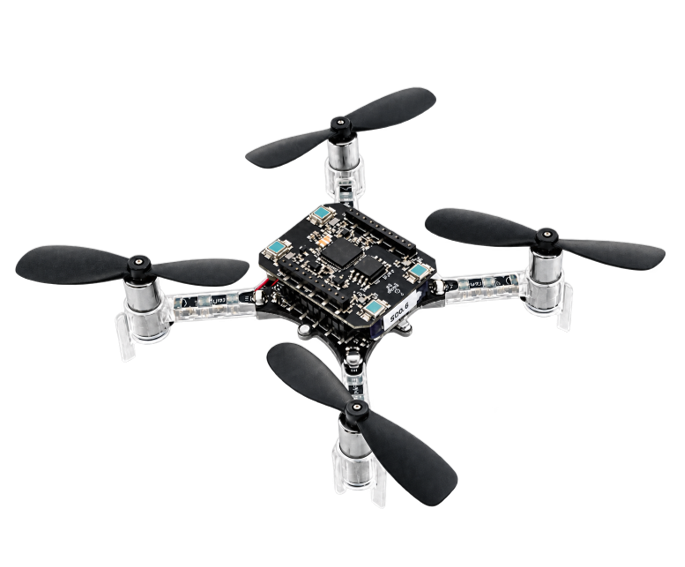
\includegraphics[height=3.08cm]{Methodology/Physical_Environment.png}};

\node[font=\bfseries\normalsize,align=center] (dtitle) at (9.0,7.70)
  {Digital Twin ($\circ$)\\[-0.2mm]{\normalfont\normalsize Objective: identify $\boldsymbol{\theta}_p$}};
\node (dimage) at (9.0,5.55)
  {
\includegraphics[height=3.08cm]{Methodology/Digital_Twin.png}};

% EXP
\node[block] (b1) at (0,2.75) {
  \textbf{Deployed policy $\pi_\bullet^{(n)}$}\\[1mm]
  $e_n=1$: information $\pi_\iota(\cdot\mid\boldsymbol{\theta}_\iota^{(n)})$\\
  $e_n=0$: performance $\pi_\bullet(\cdot\mid\boldsymbol{\theta}_\pi^{(n)})$
};

\node[block] (b2) at (0,0.35) {
  \textbf{Physical episode $n$}\\[1mm]
  state $\mathbf{s}_\bullet$, actions $\mathbf a_\bullet$, input $\mathbf z$\\
  noisy observations $\mathbf{o}_\bullet$
};

\node[block] (b3) at (0,-2.10) {
  \textbf{Record $\mathcal E^{(n)}$}\\[1mm]
  $\mathcal E^{(n)}$ stored in $\mathcal B_n$;\\
  evaluated $\mathcal R_\bullet^{(n)}$
  
};

% Digital twin
\node[block] (b6) at (9.0,2.75) {
  \textbf{Choice of the next episode}\\[1mm]
  $e_{n+1}=1$: $\mathcal J_{\mathrm{info}}
  \rightarrow\boldsymbol{\theta}_\iota^{(n+1)}$\\
  $e_{n+1}=0$: $\operatorname{EI}
  \rightarrow\boldsymbol{\theta}_\pi^{(n+1)}$\\
  {\footnotesize EI after initial surrogate calibration}
};

\node[block] (b5) at (9.0,0.35) {
  \textbf{Virtual candidate evaluation}\\[1mm]
  $e_{n+1}=1$: informativeness $\mathcal J_{\mathrm{info}}(\boldsymbol{\theta}_\iota)$
  \\
  $e_{n+1}=0$: $\pi_{\mathrm{MB}}$, candidates in $\mathcal P_n$, $\mathcal R_\circ$
};

\node[block] (b4) at (9.0,-2.10) { 
  \textbf{Factual replay}\\[1mm]
  
  initial-state reconstruction; episode replay\\
  information phase: $\overline{\mathbf o}_\circ$ vs. $\mathbf o_\bullet\rightarrow\boldsymbol{\theta}_p^{(m+1)}$\\
  performance phase: $\boldsymbol{\theta}_p$ fixed
};

% Number labels
\node[number, anchor=center] at ([xshift=-3.08cm,yshift=0.78cm]b1.center) {1};
\node[number, anchor=center] at ([xshift=-3.08cm,yshift=0.78cm]b2.center) {2};
\node[number, anchor=center] at ([xshift=-3.08cm,yshift=0.78cm]b3.center) {3};
\node[number, anchor=center] at ([xshift=-3.08cm,yshift=0.78cm]b4.center) {4};
\node[number, anchor=center] at ([xshift=-3.08cm,yshift=0.78cm]b5.center) {5};
\node[number, anchor=center] at ([xshift=-3.08cm,yshift=0.78cm]b6.center) {6};

% Main loop
\draw[flow] (b1.south) -- node[note,right]{deploy} (b2.north);
\draw[flow] (b2.south) -- node[note,right]{measure} (b3.north);
\draw[flow] (b3.east) -- node[note,below]{$\mathcal B_n$} (b4.west);
\draw[flow] (b4.north) -- node[note,right]{$\boldsymbol{\theta}_p$} (b5.south);
\draw[flow] (b5.north) -- node[note,right]{
  $\mathcal R_\circ,\,\mathcal J_{\mathrm{info}}$} (b6.south);
\draw[flow] (b6.west) -- node[note,above,text width=3.2cm,align=center]{
  next episode:\\[0.8mm] $\boldsymbol{\theta}_\pi^{(n+1)}$ or $\boldsymbol{\theta}_\iota^{(n+1)}$} (b1.east);

% Measured performance data bypasses factual identification
\draw[flow] (b3.east) -- ++(1.00,0) coordinate (retcorner)  -- node[note,rotate=90,above]{
  $\boldsymbol{\theta}_\pi^{(n)},\,\mathcal R_\bullet^{(n)}\quad(e_n=0)$} (retcorner |- b6.south west)  -- (b6.south west);

% Panel backgrounds
\begin{scope}[on background layer]
  \node[fit=(ptitle)(pimage)(b1)(b2)(b3),
        fill=black!5, draw=black!12, rounded corners=8pt,
        inner sep=10pt] {};
  \node[fit=(dtitle)(dimage)(b4)(b5)(b6),
        fill=white, draw=black!35, rounded corners=8pt,
        inner sep=10pt] {};
\end{scope}

\end{tikzpicture}%
}
\caption{Reinforcement Twinning closed loop for an episode $n$, from policy deployment to the selection of the policy for episode $n+1$. (1) Following initialization with $\pi_{\mathrm{BL}}$, an information-oriented or performance-oriented policy is deployed by supplying $\mathbf x^\ast$ to the baseline feedback controller. (2) The physical episode is performed in the presence of exogenous inputs $\mathbf z$, and observations $\mathbf o_\bullet$ are acquired. (3) The episode record $\mathcal E^{(n)}$ is stored in $\mathcal B_n$ and the physical return $\mathcal R_\bullet^{(n)}$ is evaluated. (4) The episode is replayed in the DT from reconstructed initial conditions. During the information phase, including the initial baseline replay, $\boldsymbol{\theta}_p$ is identified by comparing $\overline{\mathbf o}_\circ$ with $\mathbf o_\bullet$. During the subsequent performance phase, $\boldsymbol{\theta}_p$ is kept fixed and paired returns are obtained for surrogate calibration. (5) Candidate episodes are evaluated virtually to quantify their expected information or their DT return around $\pi_{\mathrm{MB}}$. (6) For $e_{n+1}=1$, $\boldsymbol{\theta}_\iota^{(n+1)}$ is selected by minimizing $\mathcal J_{\mathrm{info}}$; for $e_{n+1}=0$, $\pi_{\mathrm{MB}}$ and initial calibration policies are deployed first, after which further policies are selected using EI and the calibrated return transfer surrogate. In the adopted schedule, the information phase is completed first, after which the identified model is frozen during the performance phase.}
\label{fig:rt_framework} 
\end{figure*}
  
The operations carried out in each block can be summarized as follows:

(1) \textbf{Policy deployment:} the episode is started from the parameters selected at the end of the previous DT evaluation, except for the initial baseline episode, in which the nominal task reference is supplied directly to the baseline feedback controller.
For $e_n=1$, an information-oriented $\pi_\iota(\cdot\mid\boldsymbol{\theta}_\iota^{(n)})$ is deployed; for $e_n=0$, a performance-oriented $\pi_\bullet(\cdot\mid\boldsymbol{\theta}_\pi^{(n)})$ is deployed. The reference $\mathbf{x}^{\ast}$ specified by these parameters is supplied to the baseline feedback controller. A design decision made in the DT is thus converted into an executable policy, whose effectiveness is subsequently assessed in the EXP.

(2) \textbf{Physical episode:} the position reference $\mathbf{x}^{\ast}$ is supplied to the baseline feedback controller, through which the actions $\mathbf a_\bullet$ are generated and applied to the EXP. The response is affected by the exogenous input $\mathbf z$, including disturbances not selected by the policy. Although the complete $\mathbf s_\bullet$ is generally unavailable, $\mathbf o_\bullet$ is acquired together with the reference, available controller records, and operating conditions $\mathbf c$. Identification and performance assessment are consequently based on the quantities that can actually be measured. 

(3) \textbf{Recording:} the observations, deployed policy, operating conditions, control signals, available exogenous inputs, and evaluated $\mathcal R_\bullet^{(n)}$ are collected in $\mathcal E^{(n)}$ and appended to $\mathcal B_n$. The returns of $\pi_{\mathrm{BL}}$ and the subsequent performance-oriented policies are associated with their deployed $\boldsymbol{\theta}_\pi^{(n)}$ and supplied to the return transfer surrogate. Purely information-oriented episodes contribute to $\mathcal B_n$ but are excluded from surrogate calibration. 

(4) \textbf{Factual replay:} the initial conditions are reconstructed, including the internal state of the baseline feedback controller, and the recorded reference is replayed in the DT at the corresponding $\mathbf c$. During the information phase, $\overline{\mathbf o}_\circ$ is compared with $\mathbf o_\bullet$ and $\boldsymbol{\theta}_p$ is identified using the cumulative $\mathcal B_n$ through Eq.~\eqref{eq:rt-model-objective}. The same identification procedure is first applied to the initial baseline record, even though $\pi_{\mathrm{BL}}$ is a performance-oriented policy. The effect of $\boldsymbol{\theta}_p$ on the feedback response is included through the reproduced baseline feedback controller. During the subsequent performance phase, $\boldsymbol{\theta}_p$ is kept fixed, and the measured $\mathcal R_\bullet$ is paired with $\mathcal R_\circ$ to refine the return transfer surrogate. The baseline $\mathcal R_\circ$ used for calibration is reevaluated with this frozen DT.

(5) \textbf{Virtual candidate evaluation:} with the current $\boldsymbol{\theta}_p$, candidate episodes are evaluated before physical deployment. In the information phase, their predicted observations are differentiated with respect to $\boldsymbol{\theta}_p$ and scored by the information expected to be added along the weakest parameter direction. At the transition to performance, $\pi_{\mathrm{MB}}$ is computed in the identified DT. Candidate modifications around this policy are then simulated within $\mathcal P_n$, screened against the prescribed virtual constraints, and assigned $\mathcal R_\circ$. A large candidate set can therefore be evaluated in the DT while only a small subset is selected for physical testing.

(6) \textbf{Choice of the next episode:} the virtual evaluations are used to select $\boldsymbol{\theta}_\iota^{(n+1)}$ or $\boldsymbol{\theta}_\pi^{(n+1)}$ according to $e_{n+1}$. For $e_{n+1}=1$, Eq.~\eqref{eq:rt-e-optimal} is used to minimize $\mathcal J_{\mathrm{info}}$, equivalently maximizing $\lambda_{\min}[\mathbf F_{n+1}(\boldsymbol{\theta}_\iota)]$, with any additional novelty check applied as described in the information phase. For $e_{n+1}=0$, $\pi_{\mathrm{MB}}$ is deployed first, followed by the initial policies used to calibrate the surrogate from paired returns. Once this initial calibration has been completed, its predicted mean and uncertainty are used to evaluate EI, and the next $\boldsymbol{\theta}_\pi$ is selected through Eq.~\eqref{eq:rt-next-performance}. The selected parameters are returned to Block~1, $n$ is advanced, and the loop is repeated. The index $m$ is advanced only when an update of $\boldsymbol{\theta}_p$ is accepted.

Following the initial baseline episode and its first identification update, Blocks~1--6 are repeated with $e_n=1$ until the identification stopping criteria are satisfied. The identified $\boldsymbol{\theta}_p$ is then frozen, $\pi_{\mathrm{MB}}$ is deployed, and the loop is continued with $e_n=0$, first for surrogate calibration and then for EI-guided refinement. During the performance search, $\mathcal P_n$ may be extended when promising policies are found near its boundaries. The following section specializes the two environments and the associated identification and policy-design operations for the experimental application.

\section{Test Case Physical and Digital Environments}
\label{sec:setup}
\paragraph*{Experimental setup}
The experiments are designed to reproduce a transition between out-of-ground-effect (OGE) and in-ground-effect (IGE) conditions over a finite obstacle while maintaining a constant forward flight speed. The experimental setup and adopted reference frame are illustrated in Fig.~\ref{fig:experimental_setup}.

The campaign is performed using a Crazyflie 2.1+ MAV from Bitcraze flying in the $x$-$z$ plane at $y=0$~m. The horizontal reference frame retains its origin at $x=y=0$, whereas the vertical origin is placed at the upper surface of the obstacle, so that $z=0$ at the obstacle height. Positive $z$ therefore measures the vertical distance of the vehicle from this surface, and $z/R$ is the corresponding nondimensional clearance, with $R=23$~mm. Each test begins at $x=0$~m, where the MAV reaches the prescribed altitude and hovers for 10~s. It then accelerates smoothly and reaches the desired forward speed around $x=1.0$-$1.2$~m while maintaining the prescribed $z/R$. The region of interest used for comparison with the DT results spans $x=1.70$-$4.00$~m. The MAV subsequently decelerates and lands around $x=4.20$~m. Within the region of interest, the obstacle extends from $x=2.20$~m to $x=3.01$~m, corresponding to a streamwise length of $0.81$~m. In the results, the streamwise coordinate is shifted to the beginning of the region of interest and normalized by $R$; consequently, this region covers $0\leq x/R\leq100$, while the obstacle occupies approximately $21.7\leq x/R\leq57.0$.

The Crazyflie 2.1+ is equipped with an onboard IMU sensor for attitude control and a Lighthouse positioning deck for position control. Together with a 350 mAh battery, the drone mass is around $m=32.42$~g. To provide a continuous position reference, the Lighthouse deck is detected by two Lighthouse infrared stations. Their placement is selected such that the MAV remains visible to at least one station throughout the complete trajectory. In the region directly above the obstacle, which constitutes the main area of interest for the GE experiments, the fields of view of the two stations intentionally overlap. This configuration reduces the probability of temporary tracking loss or a position-estimation disturbance caused by an interruption of the optical link between a Lighthouse station and the Lighthouse deck mounted on the Crazyflie. The Lighthouse positioning system provides sub-centimetre-level absolute accuracy and sub-millimetre repeatability. In flight experiments, Taffanel et al.~\cite{Taffanel2021Lighthouse} reported an average positioning error of approximately $0.5-1$~cm and an RMS position jitter between $0.5$ and $1$~mm, depending on the adopted estimator. 

\begin{figure*}[t]
    \centering
    \definecolor{setupforestgreen}{HTML}{1B6F1B}
    \resizebox{0.98\textwidth}{!}{%
    % Match the line opacity to the drone poses by streamwise position.
    % A fitted PGF fading maps the path extent to shading coordinates 25--75 bp.
    \pgfdeclarehorizontalshading{baseline-response-opacity}{100bp}{%
        color(0bp)=(pgftransparent!40);
        color(25bp)=(pgftransparent!40);
        color(29.074bp)=(pgftransparent!40);
        color(44.074bp)=(pgftransparent!30);
        color(52.037bp)=(pgftransparent!20);
        color(63.519bp)=(pgftransparent!10);
        color(72.037bp)=(pgftransparent!0);
        color(75bp)=(pgftransparent!0);
        color(100bp)=(pgftransparent!0)}
    \pgfdeclarefading{baseline-response-fade}{\pgfuseshading{baseline-response-opacity}}
    \begin{tikzpicture}[>=Latex,font=\small]
        \path[use as bounding box] (-7.4,-2.75) rectangle (7.4,5.25);

        % Schematic, overlapping Lighthouse fields of view
        \begin{scope}[on background layer]
            \clip (-7.4,-2.75) rectangle (7.4,5.25);
            \fill[red!15,opacity=0.14] (-6.25,3.95) -- (-8.00,-2.65) -- (23.00,-2.65) -- cycle;
            \fill[red!15,opacity=0.14] ( 6.25,3.95) -- ( 8.00,-2.65) -- (-23.00,-2.65) -- cycle;
        \end{scope}

        % Lighthouse stations; station 1 uses the mirrored PNG
        \node (lh1) at (-6.25,4.15) {\reflectbox{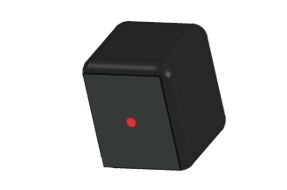
\includegraphics[width=1.45cm]{Setups/lighthouse.png}}};
        \node (lh2) at ( 6.25,4.15) {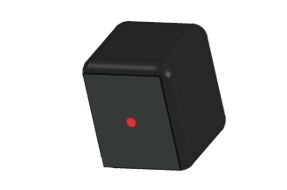
\includegraphics[width=1.45cm]{Setups/lighthouse.png}};
        \node[draw,rounded corners=2pt,fill=white,inner sep=3pt,anchor=south] at (-6.25,4.86) {Lighthouse station 1};
        \node[draw,rounded corners=2pt,fill=white,inner sep=3pt,anchor=south] at ( 6.25,4.86) {Lighthouse station 2};

        % Region of interest; streamwise annotations use its upstream origin
        \foreach \roiX in {-4.90,6.25}{
            \draw[densely dotted,setupforestgreen,line width=1.2pt] (\roiX,-1.80) -- (\roiX,3.30);
        }
        \node[setupforestgreen,anchor=north] at (-4.90,-1.89) {$x/R=0$};
        \node[setupforestgreen,anchor=north] at ( 6.25,-1.89) {$x/R=100$};

        % Constant nominal baseline reference and qualitative measured response
        \draw[densely dashed,black,line width=0.8pt] (-6.70,1.20) -- (6.80,1.20);
        \draw[black,line width=1.0pt,path fading=baseline-response-fade]
            (-6.70,1.20)
            .. controls (-5.70,1.20) and (-4.00,1.17) .. (-3.10,1.20)
            .. controls (-2.45,1.23) and (-2.35,1.85) .. (-1.55,1.91)
            .. controls (-0.95,1.93) and (-0.85,1.58) .. (0.00,1.58)
            .. controls (0.90,1.60) and (1.70,1.50) .. (2.45,1.31)
            .. controls (2.90,1.15) and (3.05,0.47) .. (3.70,0.47)
            .. controls (4.80,0.47) and (4.70,1.15) .. (5.60,1.18)
            .. controls (6.10,1.21) and (6.40,1.20) .. (6.80,1.20);
        \node[setupforestgreen,font=\normalsize,anchor=east] at (-5.05,2.95) {$v_x/v_h\rightarrow v_x^\ast/v_h$};
        \node[setupforestgreen,font=\normalsize,anchor=west] at (-4.65,2.95) {$v_x/v_h=v_x^\ast/v_h=\mathrm{const}$};

        % Vehicle poses follow the measured response, not the commanded reference
        \foreach \xx/\zz/\op in {-6.45/1.27/0.60,-3.75/1.26/0.646,-1.55/1.98/0.70,0.60/1.65/0.80,3.70/0.54/0.90,6.00/1.27/1.00}{
            \node[opacity=\op] at (\xx,\zz) {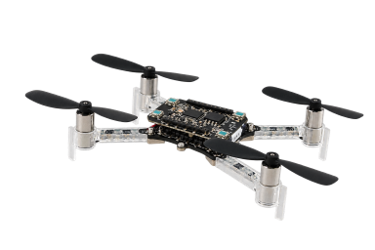
\includegraphics[width=1.55cm]{Setups/drone.png}};
        }
        \node[draw,rounded corners=2pt,fill=white,inner sep=3pt,align=center,anchor=south] at (3.10,2.20)
            {Crazyflie 2.1+ with Lighthouse deck};

        % Smaller finite obstacle; the front upper surface is at the origin height
        \node[anchor=north] (obs) at (0,0.62) {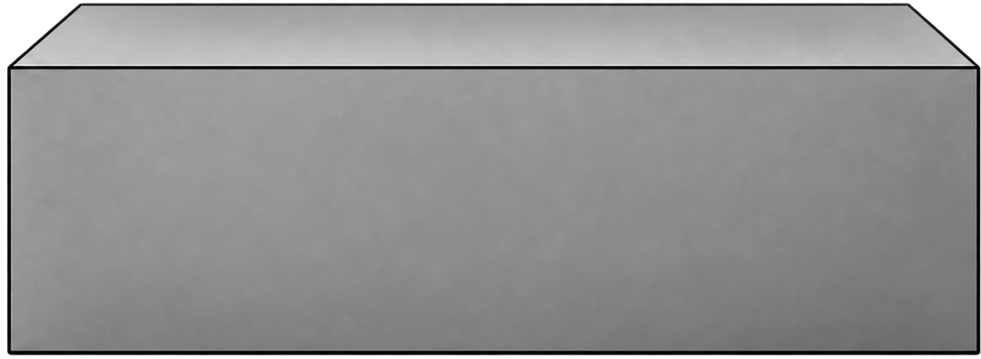
\includegraphics[width=5.20cm]{Setups/obstacle.png}};
        \node[draw,rounded corners=2pt,fill=white,inner sep=3pt] at (0,-0.50) {Finite obstacle};
        \node[black!78,anchor=north] at (-2.60,-1.59) {$x/R=22$};
        \node[black!78,anchor=north] at ( 2.60,-1.59) {$x/R=57$};
        \node[red!75!black] at (0,0.92) {Ground Effect ($T\uparrow$)};
        \draw[<->,very thick,red!75!black] (1.80,0.25) -- (1.80,1.20)
            node[midway,right] {$z^\ast/R$};

        % Reference triad on the upstream ROI boundary, at obstacle-top elevation
        \coordinate (O) at (-4.90,0.25);
        \fill (O) circle (1.4pt);
        \draw[->,thick] (O) -- ++(0.70,0) node[right] {$x_x$};
        \draw[->,thick] (O) -- ++(0,0.55) node[above right,inner sep=0.5pt,xshift=2pt] {$x_z$};
        \draw[->,thick] (O) -- ++(-0.42,-0.30) node[below left,inner sep=0.5pt] {$x_y$};
    \end{tikzpicture}%
    }
    \caption{Qualitative schematic of the experimental setup and baseline crossing (not to scale). Two Lighthouse stations provide positioning measurements, with overlapping fields of view indicated by the pale red cones. Dark-green dotted lines delimit the region of interest used for EXP--DT comparison, with the streamwise coordinate shifted to its upstream boundary: $0\leq x/R\leq100$. The finite obstacle extends from approximately $x/R=22$ to $57$, with $R=23$~mm the rotor radius. The reference-frame directions are denoted by $x_x$, $x_y$, and $x_z$; the triad is drawn on the upstream dark-green boundary at the obstacle-top elevation, which defines zero vertical clearance. The dashed black line (\mbox{-\,-}) represents the baseline policy $\pi_{\mathrm{BL}}$, which commands constant nominal clearance $z^\ast/R$ and approximately constant forward speed $v_x^\ast/v_h$. The velocity annotations distinguish acceleration toward this set point upstream of the region of interest from constant-speed crossing within it. The solid black line (\mbox{-}) represents the qualitative measured trajectory $\mathrm{EXP}_{\mathrm{BL}}$: ground effect produces an upward excursion over the obstacle and an undershoot downstream. Successive drone poses follow this measured trajectory. The opacity of the solid line and the drone poses increases downstream to indicate progression through the episode. The red double arrow measures the nominal clearance from the upper obstacle surface to the desired trajectory. The red Ground Effect annotation denotes thrust augmentation ($T\uparrow$) above the obstacle.}
    \label{fig:experimental_setup}
\end{figure*}

During each run, the Crazyflie firmware records the vehicle state, control response, and operating conditions. The logged quantities include position and translational velocity, attitude and angular rates, acceleration, battery voltage, collective-thrust command, and the individual motor PWM commands. The complete record is retained for trajectory assessment and for reconstructing each physical episode in the DT. For GE identification, the physical and DT trajectories are aligned along the streamwise coordinate, and the adjoint optimization minimizes the normalized vertical-position discrepancy over the obstacle region. The remaining channels support initialization and replay of the measured operating conditions, but do not enter the identification objective directly.

The Crazyflie is operated using its standard cascaded PID control architecture, as documented by Bitcraze~\cite{BitcrazeControllers}. An outer position loop tracks the commanded position $\mathbf{x}_{\pi}^{\ast}$ and generates the corresponding velocity reference $\mathbf{v}_{\pi}^{\ast}$. For the baseline policy, $\mathbf{x}_{\pi}^{\ast}=\mathbf{x}^{\ast}$; the optimized policies modify the commanded vertical coordinate while retaining the nominal tracking objective $\mathbf{x}^{\ast}$. A velocity loop then regulates the translational motion, producing the desired roll and pitch angles together with the collective thrust command. These references are passed to the attitude controller, which determines the desired body angular rates. Finally, the inner angular-rate controller generates the roll, pitch, and yaw control contributions, which are combined with the collective thrust through the onboard motor mixer to determine the four individual motor commands. The same control architecture and firmware logic are reproduced in the DT from the official implementation~\cite{BitcrazeFirmware}, ensuring consistency between the numerical and experimental closed-loop dynamics.

\paragraph*{Digital Twin}
\label{sec:digital_twin}

The Digital Twin developed in this work follows the modeling formulation proposed by Richardson et al.~\cite{Richardson2025} for low-speed free flight and is tailored to reproduce the dynamics of the Crazyflie 2.1+ employed in the experimental campaign. The model is implemented as a differentiable physics-based simulator using the JAX library in Python and is used for both model identification and control optimization. The vehicle kinematics, rigid-body dynamics, propulsion system, battery dependence, actuator dynamics, and cascaded controller together form the nominal starting DT. Their parameters are inherited unchanged from Richardson et al.; they are neither reidentified nor independently revalidated in the present campaign. The finite-obstacle ground-effect correction is incorporated below as the unknown model component with associated $\boldsymbol{\theta}_p$ learned by RT.

The Crazyflie is modeled as a six-degree-of-freedom rigid body. The position $\mathbf{x}=[x,y,z]^{\mathsf T}$ and translational velocity $\mathbf{v}=[v_x,v_y,v_z]^{\mathsf T}$ are expressed in the inertial frame, while the attitude is represented by the quaternion $\mathbf{q}=[q_w,q_x,q_y,q_z]^{\mathsf T}$ and the body angular velocity by $\boldsymbol{\omega}=[\omega_x,\omega_y,\omega_z]^{\mathsf T}$. Together with the rotor speeds $\Omega_i$, these quantities describe the vehicle response within $\mathbf s_\circ$; the complete closed-loop simulation also propagates the actuator and controller memory.

The translational dynamics evaluated at the center of mass (CoM) are
%
\begin{equation}
\begin{cases}
{\dot{\mathbf{x}}=\mathbf{v}}\\
{m\dot{\mathbf{v}}=m\mathbf{g}+\mathbf{R}\mathbf{F}_{B}}
\end{cases}
\label{eq_vehicle_trasl}
\end{equation}
where $\mathbf{g}=[0,0,-g]^T$, $g$ is the gravitational acceleration, and $\mathbf{R}\in SO(3)$ transforms quantities from the body-fixed frame to the inertial frame. The total force in body coordinates is $\mathbf{F}_{B}=[0,0,T]^T$, where $T$ is the total thrust generated by the four rotors.
%

The rotational dynamics follow Euler's rigid-body equation,
%
\begin{equation}
\mathbf{I}\dot{\boldsymbol{\omega}}
+
\boldsymbol{\omega}
\times
(\mathbf{I}\boldsymbol{\omega})
= \boldsymbol{\tau}
\label{eq_vehicle_rot}
\end{equation}
where $\mathbf{I}$ is the inertia tensor and $\boldsymbol{\tau}=[\tau_x,\tau_y,\tau_z]^T$ is the total moment vector expressed in body coordinates.
%
The vehicle attitude is propagated through the unit quaternion according to
%
\begin{equation}
\dot{\mathbf q} = \frac{1}{2}
\mathbf{\Lambda}(\boldsymbol{\omega})\mathbf q
\label{eq_vehicle_attitude}
\end{equation}
where $\mathbf{\Lambda}(\boldsymbol{\omega})$ is the scalar-first quaternion kinematic matrix associated with the body angular velocity, using the convention adopted by Richardson et al.~\cite{Richardson2025}.
%
The thrust and reaction torque generated by rotor $i$ are modeled as
%
\begin{equation}
\begin{cases}
{T_i=k_T\Omega_i^2}\\
{Q_i=k_Q\Omega_i^2}
\end{cases}
\label{eq_T_and_Q}
\end{equation}
where $T_i$ and $Q_i$ are the individual rotor thrust and torque and $k_T$ and $k_Q$ are the corresponding coefficients. The total thrust and moments follow from their signed combination.
%
For the adopted quadcopter and motor convention, the roll ($\tau_R$), pitch ($\tau_P$), and yaw ($\tau_Y$) moments are
%
\begin{equation}
\begin{cases}
{\tau_R=
\frac{d}{2}
\left(
-T_1-T_2+T_3+T_4
\right)}\\
{\tau_P=
\frac{d}{2}
\left(
-T_1+T_2+T_3-T_4
\right)}\\
{\tau_Y=
\sum_{i=1}^{4}s_iQ_i,}
\end{cases}
\label{eq_RP_moments}
\end{equation}
where $d$ is the motor-to-motor distance and $s_i\in\{-1,+1\}$ identifies the rotation direction of rotor $i$.
%

The connection between the motor commands and propeller speed follows the Crazyflie propulsion characterization adopted by Richardson et al. The effect of battery state is included through the battery voltage $V_b=f(\mathrm{SOC})$, where $\mathrm{SOC}$ denotes the battery state of charge. A voltage correction factor is defined as $\eta_V=V_b/V_{\mathrm{ref}}$, where $V_{\mathrm{ref}}$ is the voltage of a fully charged battery. The rotor-speed command associated with the PWM input is corrected as $\Omega_{\mathrm{cmd}}=\eta_V\Omega_{\mathrm{PWM}}$. The realized rotor speed follows this command through a first-order actuator model with time constant $\tau_{\mathrm{rpm}}=0.020$~s. This value is inherited from the Richardson model and is not identified in the present work.

The main physical parameters adopted in the DT are taken from the formulation of \cite{Richardson2025} and are summarized in Table~\ref{tab:dt_parameters}. The nominal propulsion model retains the battery-voltage correction $V_b=f(\mathrm{SOC})$. However, both physical and DT missions start with a fully charged battery and last only a few seconds; therefore, the within-mission change of state of charge is neglected. The vehicle dynamics are coupled with the same cascaded PID architecture used in the physical environment, providing the nominal closed-loop model on which the ground-effect correction is identified.
\begin{table}[t]
\centering
\caption{Baseline DT parameters adopted from Richardson et al.~\cite{Richardson2025}.}
\label{tab:dt_parameters}
\begin{tabular}{lc}
\hline
Parameter & Value \\
\hline
$m$ & $0.03242$ kg\\
$R$ & $0.023$ m \\
$d$ & $0.065$ m \\
$I_{xx}$ & $16.57\times10^{-6}$ kg m$^2$ \\
$I_{yy}$ & $16.56\times10^{-6}$ kg m$^2$ \\
$I_{zz}$ & $29.26\times10^{-6}$ kg m$^2$ \\
$k_T$ & $2.88\times10^{-8}$ N s$^2$/rad$^2$ \\
$k_Q$ & $7.24\times10^{-10}$ N m s$^2$/rad$^2$ \\
$\tau_{\mathrm{rpm}}$ & $0.020$ s \\
$V_{\mathrm{ref}}$ & $4.20$ V \\
\hline
\end{tabular}
\end{table}
\paragraph*{Ground-effect correction}
\label{sec:ge-model}
The described nominal DT reproduces the vehicle dynamics in free flight and was validated in those conditions by Richardson et al.~\cite{Richardson2025}. The nominal DT, however,  does not account for the additional rotor-surface interaction generated as the vehicle closely crosses the finite obstacle. This interaction is introduced through a deliberately simple physical model inspired by the analytical formulation of Cheeseman and Bennett for an isolated rotor in hovering~\cite{CheesemanBennett1955}. For a rotor $i$ of radius $R$ at a clearance $z_i$ from the obstacle, the in-ground-effect thrust $T_{i,\mathrm{IGE}}$ is obtained from the nominal out-of-ground-effect thrust $T_{i,\mathrm{OGE}}$ through the amplification factor $f_{\mathrm{GE}}$,
\begin{equation}
 T_{i,\mathrm{IGE}}
 =T_{i,\mathrm{OGE}}\,
 f_{\mathrm{GE}}(z_i;\boldsymbol{\theta}_p).
 \label{eq:ge-thrust-factor}
\end{equation}
The amplification factor is modeled as
\begin{equation}
 f_{\mathrm{GE}}(z_i;\boldsymbol{\theta}_p)=1+A\left(\frac{R}{z_i}\right)^p,
 \qquad \boldsymbol{\theta}_p=[A,\,p]^\top .
 \label{eq:fge}
\end{equation}
Here, $A$ controls the magnitude of the thrust augmentation, while $p$ determines how rapidly the interaction decays with increasing clearance. The original Cheeseman and Bennett formulation rearranged with the same unknowns would have retained $A=1/16$ and $p=2$. These values initialize the identification in the present work, while both coefficients remain free to adapt to the present vehicle and operating conditions.

This model is deliberately low order: ground effect is treated as a static function of the instantaneous rotor clearance. Measurements by Kan et al.~\cite{Kan2019} indicate that velocity dependence is limited over the low-speed range considered here, but it is not assumed to vanish. The formulation also omits the transient development and decay of the rotor-surface interaction as the vehicle crosses the obstacle edges. These omissions preserve a compact model that can be identified and differentiated efficiently, while leaving a structural discrepancy that is addressed later through the reward-transfer surrogate.

Equation~\eqref{eq:fge} describes the clearance dependence above an extended surface. The obstacle considered here occupies only a finite streamwise interval, so the augmentation must also depend on the position of each rotor relative to its edges. It is therefore weighted by $\chi_i(x)\in[0,1]$, defined as the fraction of rotor disk $i$ that overlaps the obstacle. The corrected rotor thrust becomes
\begin{equation}
 T_{i,\mathrm{corr}}=T_{i,\mathrm{OGE}}\left[1+\chi_i(x)\left(f_{\mathrm{GE}}(z_i;\boldsymbol{\theta}_p)-1\right)\right],
 \label{eq:corrected-thrust}
\end{equation}
where $T_{i,\mathrm{OGE}}$ is the nominal rotor thrust outside ground effect. The overlap fraction is zero when the rotor lies outside the obstacle footprint and reaches unity when its disk is fully above it. Its continuous variation across the leading and trailing edges avoids discontinuous force changes and naturally accounts for the four rotors entering and leaving the obstacle region at different streamwise positions. 

\subsection{Test Campaign Overview}
\label{sec:test-campaign}
Following Kan et al.~\cite{Kan2019}, the desired forward velocity is normalized by the ideal induced velocity in hover,
\begin{equation}
 v_h=\sqrt{\frac{T_{h,r}}{2\rho_a\pi R^2}}
 =\sqrt{\frac{mg}{8\rho_a\pi R^2}},
 \label{eq:hover-induced-velocity}
\end{equation}
where $T_{h,r}=mg/4$ is the hover thrust required from each rotor, $\rho_a$ is the air density, and $R$ is the rotor radius. With $m=32.42$~g, $R=0.023$~m, and $\rho_a=1.225$~kg/m$^3$, Eq.~\eqref{eq:hover-induced-velocity} gives $v_h\simeq4.42$~m/s. An operating condition is henceforth denoted by the ordered pair $(z^\ast/R,\,v_x^\ast/v_h)$.

The test campaign follows the sequential RT schedule introduced above. All tests use the same physical environment, DT structure, reference frame, and data-processing procedure described in Sec.~\ref{sec:setup}. The nominal operating condition is $(z^\ast/R,\,v_x^\ast/v_h)=(1.5,0.079)$. Unless stated otherwise, policy design, model identification, and reward evaluation refer to this condition. The campaign is organized into five consecutive blocks, introduced below together with the notation used in the results.

\paragraph*{\textit{Baseline policy}}
The campaign starts from the built-in cascaded PID controller at the nominal condition $(z^\ast/R,\,v_x^\ast/v_h)=(1.5,0.079)$. This policy is denoted by $\pi_{\mathrm{BL}}$ and is repeated experimentally to quantify run-to-run variability. Its mean response and RMS band provide the reference trajectory statistics, the first record in the replay buffer, and the baseline tracking cost used to normalize the rewards reported later. Since $\pi_{\mathrm{BL}}$ reacts only after the vehicle departs from the desired clearance, it also exposes the ground-effect excursion that the subsequent predictive policies are designed to anticipate.

\paragraph*{\textit{Information phase}}
\label{sec:information-phase}
The objective of the information phase is to design and perform trajectories that improve the identification of the unknown parameters $\boldsymbol{\theta}_p=[A,p]$ of the ground-effect model described by Eqs.~\eqref{eq:ge-thrust-factor} and~\eqref{eq:fge}.
Each trajectory deployed in the physical environment is replayed through the differentiable DT with the same reference and reconstructed initial condition used experimentally. Factual replay identifies the coefficient pair from the accumulated tracking response. The subsequent DT design searches for a safe altitude reference that adds information along the least-observed parameter direction, thereby defining the next experiment. The two operations are repeated sequentially, with each new flight updating both the identified parameters and the information available for the next design.

The model is initialized from the Cheeseman-Bennett coefficients, $A=1/16$ and $p=2$. Starting from the baseline record, twelve information-oriented policies $\pi_{\mathrm{INF}}^{(n)}$ are added sequentially to the cumulative dataset. The first six policies are designed over the broad admissible clearance range $0.5<z/R<6$. This first stage deliberately explores a wide set of altitude histories: it establishes the global scale and decay of the interaction without assuming in advance that the most useful data must come from the smallest admissible clearance, and it verifies the response of the evolving DT over the complete safe operating range.

By the end of the sixth information-oriented episode, new policies in the broad domain still increase the cumulative Fisher information, but their marginal E-optimal contribution has become modest compared with the first information-oriented interaction. This behavior is physically consistent with Eq.~\eqref{eq:fge}: at larger clearances, $f_{\mathrm{GE}}$ approaches unity and its sensitivity to both $A$ and $p$ decreases. The admissible design domain is therefore restricted to $0.5<z/R<1.5$ for the remaining six policies, defining the near-wall domain. The restriction is an adaptive design decision, not a rejection of the broad-domain data. All preceding episodes remain in the replay buffer, while the new candidates concentrate the available experimental effort where the identified law is steepest and the weak parameter direction can be excited more effectively. After every flight, the new record is appended to the cumulative dataset and the identification is warm-started from the preceding converged coefficients.

The information phase begins with factual replay and adjoint identification. For physical episode $n$, the experimental record provides the measured altitude-tracking error, the deployed reference policy, and the reconstructed initial condition. The DT replays the same episode with the current model parameters $\boldsymbol{\theta}_p$. The experimental and virtual error histories are evaluated at the same $K_n$ spatial positions encountered during the flight and collected in the vectors
\begin{align}
 \mathbf e_{z,n}^{\bullet}
 &=\bigl[e_{z,n}^{\bullet}(x_{n,1}),\ldots,
 e_{z,n}^{\bullet}(x_{n,K_n})\bigr]^{\mathsf T},\\
 \mathbf e_{z,n}^{\circ}(\boldsymbol{\theta}_p)
 &=\bigl[e_{z,n}^{\circ}(x_{n,1};\boldsymbol{\theta}_p),\ldots,
 e_{z,n}^{\circ}(x_{n,K_n};\boldsymbol{\theta}_p)\bigr]^{\mathsf T}.
 \label{eq:episode-error-vectors}
\end{align}
With $N$ episodes in the replay buffer, the identification loss is
\begin{equation}
 J_p(\boldsymbol{\theta}_p)=
 \frac{1}{N}\sum_{n=1}^{N}
 \frac{1}{K_n}
 \left\|
 \frac{\mathbf e_{z,n}^{\circ}(\boldsymbol{\theta}_p)
       -\mathbf e_{z,n}^{\bullet}}{R}
 \right\|_2^2.
 \label{eq:identification-loss}
\end{equation}
The factor $1/K_n$ gives every episode equal weight irrespective of its number of samples or duration.

The loss is minimized by differentiating the complete time-discrete closed-loop rollout in reverse mode. This is the discrete-adjoint formulation of the identification problem: the loss sensitivity is propagated backward through the vehicle dynamics, actuator model, controller states, and ground-effect correction. At optimization step $t$, the resulting gradient is
\begin{equation}
 \mathbf{g}_t=
 \nabla_{\boldsymbol{\theta}_p}J_p
 \bigl(\boldsymbol{\theta}_{p,t}\bigr)
 =
 \begin{bmatrix}
 \dfrac{\partial J_p}{\partial A} &
 \dfrac{\partial J_p}{\partial p}
 \end{bmatrix}^{\mathsf T}.
 \label{eq:adjoint-gradient}
\end{equation}
It accounts for the direct influence of $A$ and $p$ on the aerodynamic forces and for the trajectory changes produced through the closed feedback loop. Both derivatives are obtained in one backward pass, without a separate perturbed simulation for each parameter.

Adam uses this gradient to update the parameters over successive optimization steps. It retains a first moment $\mathbf{m}_t$, which smooths the gradient direction, and a second moment $\mathbf{v}_t$, which tracks its component-wise squared magnitude:
\begin{align}
 \mathbf{m}_t &=
 \beta_1\mathbf{m}_{t-1}
 +(1-\beta_1)\mathbf{g}_t,\\
 \mathbf{v}_t &=
 \beta_2\mathbf{v}_{t-1}
 +(1-\beta_2)\mathbf{g}_t^{\odot 2}.
 \label{eq:adam-moments}
\end{align}
The two moments allow the step size to adapt separately to $A$ and $p$, whose gradients can have different scales. After the standard bias correction, the next parameter vector is
\begin{equation}
 \boldsymbol{\theta}_{p,t+1}=
 \Pi_{\Theta}\!\left[
 \boldsymbol{\theta}_{p,t}
 -\eta
 \frac{\widehat{\mathbf{m}}_t}
 {\sqrt{\widehat{\mathbf{v}}_t}+\epsilon}
 \right],
 \label{eq:adjoint-adam}
\end{equation}
where $\eta$ is the chosen learning rate, $\epsilon$ prevents division by zero, and $\Pi_{\Theta}$ keeps the solution inside the physically admissible set $\Theta$. In the present campaign, $\eta=5\times10^{-3}$ and convergence is assessed over windows of 25 optimization steps. The relative-loss, coefficient-range, and projected-gradient tolerances are $2\times10^{-4}$, $10^{-3}$, and $5\times10^{-3}$, respectively. The optimization is considered converged only when all three conditions remain satisfied over a complete monitoring window. When a new physical episode is added, the next fit is warm-started from the previously converged parameters, while the Adam moments are reset because the cumulative objective has changed.

The converged estimate $\widehat{\boldsymbol{\theta}}_p$ is then used to determine which experiment should be performed next. Local parameter uncertainty is approximated from the curvature of the identification loss. Let
\begin{equation}
 \mathbf H=\nabla^2J_p(\widehat{\boldsymbol{\theta}}_p)
 =\mathbf Q\operatorname{diag}(\lambda_1,\lambda_2)\mathbf Q^{\mathsf T}.
\end{equation}
To avoid a singular inverse along a locally flat direction, the eigenvalues are floored at $\lambda_H=10^{-6}$. The resulting local inverse-Hessian approximation is
\begin{equation}
 \boldsymbol{\Sigma}_{\theta}\simeq
 \max\!\left[J_p(\widehat{\boldsymbol{\theta}}_p),10^{-12}\right]
 \mathbf Q\operatorname{diag}\!\left[
 \max(\lambda_1,\lambda_H)^{-1},
 \max(\lambda_2,\lambda_H)^{-1}
 \right]\mathbf Q^{\mathsf T}.
 \label{eq:parameter-covariance}
\end{equation}
This matrix is used as a local curvature-based uncertainty approximation, not as a calibrated finite-sample confidence region. A flat direction of the loss produces a larger local uncertainty. For a model output $g(\boldsymbol{\theta}_p)$, such as $f_{\mathrm{GE}}$ at a prescribed clearance, the corresponding linearized uncertainty indicator is
\begin{equation}
 \sigma_g^2=
 \nabla_{\boldsymbol{\theta}_p}g^{\mathsf T}
 \boldsymbol{\Sigma}_{\theta}
 \nabla_{\boldsymbol{\theta}_p}g.
 \label{eq:uncertainty-propagation}
\end{equation}
Thus, $A$ and $p$ may retain a strongly elongated and correlated local uncertainty region even when the resulting ground-effect curve is tightly constrained. The quantity $2\sigma_{f_{\mathrm{GE}}}/f_{\mathrm{GE}}$ reported later is the propagated relative uncertainty of the total thrust factor. It is not interpreted as an exact 95\% confidence interval, and its decrease at large clearance partly reflects that $f_{\mathrm{GE}}\rightarrow1$.

Candidate altitude-reference policies are then generated inside the admissible design space and simulated with the converged DT. Because $A$ and $p$ have different numerical scales, the sensitivity columns are normalized with the local parameter scales
\begin{equation}
 \mathbf D_{\theta}=\operatorname{diag}
 \left(\sqrt{[\boldsymbol{\Sigma}_{\theta}]_{AA}},
       \sqrt{[\boldsymbol{\Sigma}_{\theta}]_{pp}}\right),
 \qquad
 \overline{\mathbf S}_n=
 \frac{\partial\mathbf e_{z,n}^{\circ}}
 {\partial\boldsymbol{\theta}_p}\mathbf D_{\theta}.
\end{equation}
The eigenvalues can therefore be interpreted for perturbations of one local parameter standard deviation, rather than being dominated by the raw numerical scale of either coefficient. Under an independent, homoscedastic residual approximation, a common normalized residual variance is estimated as $\sigma_e^2=\max[J_p(\widehat{\boldsymbol{\theta}}_p),10^{-12}]$. The Fisher-information proxy accumulated from the $N$ completed experiments is
\begin{equation}
 \mathbf F_{1:N}=
 \sum_{n=1}^{N}
 \frac{\overline{\mathbf S}_n^{\mathsf T}\overline{\mathbf S}_n}
 {K_n\sigma_e^2},
 \label{eq:cumulative-fisher}
\end{equation}
where $K_n$ prevents a longer episode from appearing more informative solely because it contains more samples. Large eigenvalues of $\mathbf F_{1:N}$ correspond to locally scaled parameter combinations that the accumulated experiments constrain strongly; its smallest eigenvalue describes the least-observed joint parameter direction. Since spatial residuals can remain correlated, this matrix is used as a comparative design metric rather than as an exact statistical Fisher matrix. During sequential design it is evaluated with the current converged DT. For the post-campaign comparison reported later, every episode and the repeated-baseline counterfactual are reevaluated using the final DT, final parameter scaling, and the same residual variance, so their cumulative values are directly comparable.

Each virtual candidate policy $\pi$ produces a predicted Fisher contribution $\mathbf F(\pi)$. The next information-oriented policy is selected with the E-optimal criterion
\begin{equation}
 \pi_{\mathrm{INF}}^{(N+1)}=
 \arg\max_{\pi\in\Pi_{\mathrm{safe}}}
 \lambda_{\min}\!\left(
 \mathbf F_{1:N}+\mathbf F(\pi)
 \right),
 \label{eq:e-optimal-design}
\end{equation}
which selects the safe candidate predicted to increase the Fisher information along its weakest direction. The criterion already favors sensitivities that complement the accumulated dataset. A separate novelty check may nevertheless select a slightly less informative candidate when its predicted response is sufficiently different from the experiments already performed. Candidates that violate state, reference-rate, acceleration, actuator, or clearance constraints are discarded before deployment.

After the selected flight, its record is added to the replay buffer and the adjoint-Adam identification is repeated. The inner Adam loop is stopped by the numerical convergence conditions defined above. The complete information phase is terminated only when adding new episodes no longer changes the converged values of $A$ and $p$ appreciably and no longer produces a meaningful reduction in the magnitude of their estimated correlation.

\paragraph*{\textit{Model-based policy}}
\label{sec:mb-optimum}
After identification, $A$ and $p$ are frozen and the specialized performance loop uses the converged DT to improve altitude tracking across the finite obstacle. The control policy is implemented as a spatial reference governor above the unchanged cascaded PID controller, so the computationally expensive prediction and optimization remain offline while the deployed policy is a lightweight lookup table. First the DT produces the model-based policy $\pi_{\mathrm{MB}}$; physical rewards around that policy then train the reward-transfer surrogate used by Expected Improvement to design improved policies. The policy is the spatial altitude reference supplied to the governor,
\begin{equation}
 z_{\pi}(x)=z_{\mathrm{BL}}(x)+\Delta z_{\pi}(x),
 \label{eq:policy}
\end{equation}
where $z_{\mathrm{BL}}$ is the nominal mission reference altitude which is constant along $x$. The governor modifies only the vertical set point as a function of measured longitudinal position. The horizontal trajectory, attitude stabilization, motor mixing, and onboard PID gains remain unchanged. This spatial representation is preferred over the time representation as it prevents small DT-experiment timing differences from desynchronizing the anticipatory command from the obstacle.

At the nominal operating condition, the reference correction is parameterized at control points separated by one rotor radius, $\Delta x=R$, over the complete crossing and interpolated between consecutive points. Its amplitude is bounded by $|\Delta z|\leq3R$, while the predicted lowest rotor must retain a clearance of at least $0.5R$ from the local surface.

The model-based policy is first obtained through model-predictive reference synthesis.
The model-based policy $\pi_{\mathrm{MB}}$ is obtained from a finite-horizon nonlinear prediction of the complete closed-loop mission. At every optimizer step, the DT propagates the vehicle, propulsion, aerodynamic model, PID states, and reference governor over the entire prediction interval. Reverse-mode differentiation supplies the gradient with respect to all spatial reference values, and Adam updates their amplitudes subject to bound and endpoint projections. The optimized policy is therefore computed before the flight and then executed online as a lightweight interpolation table. In this work, \emph{model predictive control} refers to this model-predictive reference synthesis; a receding-horizon optimizer is not run onboard.

Performance is evaluated against the original mission reference used by the nominal cascaded PID controller. The tracking cost and corresponding reward are
\begin{equation}
 J_{\mathrm{trk}}(\pi)=\frac{1}{N_{\mathcal R}}
 \sum_{x_k\in\Omega_{\mathcal R}}
 \left[\frac{z_k-z_{\mathrm{BL}}(x_k)}{R}\right]^2,
 \qquad
 \mathcal{R}(\pi)=1-J_{\mathrm{trk}}(\pi).
 \label{eq:reward}
\end{equation}
The reported policy is optimized with the single final identified DT; no model-uncertainty ensemble is used. The objective augments the tracking term with amplitude, curvature, and clearance penalties,
\begin{align}
 J_{\mathrm{MB}}=&\;J_{\mathrm{trk}}
 +0.10\left\|\frac{\Delta z_{\pi}}{R}\right\|_2^2
 +2.0\left\|\mathbf{D}^2\frac{\Delta z_{\pi}}{R}\right\|_2^2 \notag\\
 &+10^5\Phi_{\mathrm{clr}}(\pi),
 \label{eq:mb-objective}
\end{align}
where $\mathbf{D}^2$ is the spatial second-difference operator and $\Phi_{\mathrm{clr}}$ is the mean squared violation of the $0.5R$ minimum clearance of the lowest rotor while it is above the obstacle. The amplitude term limits control authority, the curvature term suppresses spatially sharp commands, and the clearance term enforces safety on the tilted rotor geometry rather than only on the vehicle center of mass. The final policy is replayed once more in the DT and rejected if the hard clearance check fails.

\paragraph*{\textit{Performance phase}}
\label{sec:performance-phase}
The performance search is conducted at the nominal operating condition with the identified parameters frozen. Two interpolation policies, denoted collectively by $\pi_{\lambda,i}$ with $\lambda\in\{1/3,2/3\}$, are first tested between $\pi_{\mathrm{BL}}$ and $\pi_{\mathrm{MB}}$ to establish the global relation between the DT and physical rewards. The search is then expanded around $\pi_{\mathrm{MB}}$ using three smooth spatial basis functions. A scrambled Sobol library of 2000 coefficient vectors is screened in the DT, and seven admissible, mutually distinct policies $\pi_{\mathbf a,i}$ are deployed to train the local GP discrepancy. Subsequent policies $\pi_{\mathrm{EI},i}$ are selected sequentially by Expected Improvement; after each flight, the physical reward is appended to the reward-transfer surrogate dataset. The policy with the largest nominal-condition physical reward is denoted by $\pi_{\mathrm{EI}}^{\star}$.

Physical rewards are then used to refine this model-based policy and compensate for the remaining model discrepancy. Reinforcement Twinning uses these measurements to correct the local policy ranking predicted by the DT. A new candidate is written as
\begin{equation}
 \Delta z_{\pi}(x)=\Delta z_{\mathrm{MB}}(x)+
 R\,\mathbf{b}^{\mathsf T}(x)\mathbf a,
 \label{eq:rt-policy}
\end{equation}
where the smooth basis functions $\mathbf{b}(x)$ span the control-relevant portions of the mission and $\mathbf a=[a_A,a_B,a_C]^\top$ is the bounded vector of policy-modification coefficients. A space-filling library is first evaluated in the DT; the same reference and rotor-clearance checks used for the MB solution define the admissible set $\mathcal A_{\mathrm{safe}}$.

The affine component of the reward-transfer surrogate is fitted by ordinary least squares to the paired DT and physical rewards. The residual is modeled by a zero-mean Mat\'ern-$3/2$ GP. At the nominal operating condition, its input is the three-component vector $\mathbf a$, with each coordinate scaled by $0.30R$. The signal variance is initialized from the empirical variance of the affine residuals and is bounded below by $0.05^2$. The rewards are computed from the cleaned mean trajectories and are treated as deterministic campaign observations; a diagonal jitter of $10^{-8}$ is added only for numerical stability. Accordingly, the GP posterior standard deviation quantifies interpolation uncertainty within this surrogate and not run-to-run experimental dispersion. The resulting relation is
\begin{equation}
 \mathcal{R}_{\bullet}=
 \gamma_0+\gamma_1\mathcal{R}_{\circ}
 +\delta(\mathbf a,\boldsymbol{\chi})+\varepsilon,
 \label{eq:reward-transfer}
\end{equation}
where $\delta$ is the GP discrepancy and $\boldsymbol{\chi}$ contains optional operating conditions expressed by $(z^\ast/R,\,v_x^\ast/v_h)$. Two policies with similar DT performance can receive different physical corrections. Its posterior mean and variance are updated after every performance-oriented episode. Expected Improvement is used with zero exploration margin, $\xi=0$, and selects the next experiment,
\begin{align}
 Z(\mathbf a)&=
 \frac{\mu_{\bullet}(\mathbf a)-\mathcal{R}_{\bullet}^{+}}
 {\sigma_{\bullet}(\mathbf a)},\\
 \operatorname{EI}(\mathbf a)&=
 \left(\mu_{\bullet}-\mathcal{R}_{\bullet}^{+}\right)\Phi(Z)
 +\sigma_{\bullet}\phi(Z),\\
 \mathbf a_{n+1}&=
 \arg\max_{\mathbf a\in\mathcal A_{\mathrm{safe}}}
 \operatorname{EI}(\mathbf a),
 \label{eq:ei}
\end{align}
with zero improvement assigned to a vanishing posterior variance. The first term exploits candidates with a high predicted physical reward, whereas the second rewards unresolved but potentially useful regions. The model-based policy remains the reference throughout the search; data are used to learn the GP discrepancy that affects physical performance.

For transfer across operating conditions, the DT and physical performance are normalized by the corresponding condition-specific baseline cost,
\begin{equation}
 \mathcal S=1-\frac{J_{\pi}}{J_{\mathrm{BL}}}
   =1-\frac{1-\mathcal R_{\pi}}{1-\mathcal R_{\mathrm{BL}}},
 \label{eq:normalized-score}
\end{equation}
and $\boldsymbol{\chi}$ is augmented with the operating condition. Policy coordinates are defined relative to the local MB deformation. Consequently, a correction learned where the model-based action is large is reduced automatically when the local MB solution requires little intervention, rather than being transferred as a fixed altitude offset.

\paragraph*{\textit{Generalization}}
The final block evaluates whether the policy structure learned at the nominal condition remains useful when the operating condition changes. Two off-nominal conditions are considered: $(z^\ast/R,\,v_x^\ast/v_h)=(2.5,0.045)$ and $(1,0.113)$. For each condition, a baseline policy $\pi_{\mathrm{BL}}$ and a model-based policy $\pi_{\mathrm{MB}}$ are computed with the frozen identified DT. The best nominal RT correction is then transferred in the coordinates of the condition-specific model-based reference correction and denoted by $\pi_{\mathrm{EI}}^{\mathrm{tr}}$. Where an additional condition-specific EI search is performed, its best physical policy is denoted by $\pi_{\mathrm{EI}}^{\star}$. These tests distinguish direct transfer of the nominal correction from a local, proof-of-concept extension of the RT search at a new operating condition; they do not constitute convergence of a surrogate over the full velocity-clearance domain.


\section{Results and Discussion}
\label{sec:results}

\subsection{Baseline Response}
\label{sec:results-bl}

The first experimental case employs only the cascaded PID controller available in the original Crazyflie firmware. The most direct target for this baseline crossing is a constant-clearance trajectory at $(z^\ast/R,\,v_x^\ast/v_h)=(1.5,0.079)$. The desired trajectory is therefore the straight horizontal line denoted by $\pi_{\mathrm{BL}}$ and reported with a dashed line in Fig.~\ref{fig:stage0}. This case establishes the performance baseline because the controller acts exclusively through feedback, without any anticipation of the approaching aerodynamic interaction.

The solid line in Fig.~\ref{fig:stage0} reports the mean experimental trajectory $\mathrm{EXP}_{\mathrm{BL}}$ obtained from five repetitions, while the surrounding shaded region represents the corresponding $\pm\mathrm{RMS}$ run-to-run dispersion. At each streamwise position, this quantity is defined as $\mathrm{RMS}(x)=[N_r^{-1}\sum_{j=1}^{N_r}(z_j(x)-\overline z(x))^2]^{1/2}$, with $N_r=5$. The band therefore describes repeatability about the measured mean and is not an uncertainty interval for that mean. Before reaching the obstacle, the vehicle maintains an almost constant clearance close to the commanded value, supporting satisfactory tracking at this modest forward speed away from the surface interaction. The response changes markedly over the obstacle: the vehicle initially rises to approximately $z/R=2.5$ and subsequently settles around $z/R=2$. The additional thrust generated in ground effect produces the initial overshoot. The feedback controller reacts by reducing the motor speeds and commanded thrust, but this corrective action is insufficient to recover $z^\ast/R=1.5$ while the vehicle remains over the obstacle. The cascaded PID is tuned around hovering and contains no model that can anticipate the surface-induced thrust augmentation.

The opposite transient occurs at the trailing edge. Ground-effect augmentation disappears while the motor command is still reduced by the preceding feedback action, producing an undershoot down to approximately $z/R=0.5$. The vehicle then gradually recovers the commanded clearance, which is reached only about $40R$ downstream of the obstacle. Both excursions are substantially larger than the run-to-run dispersion, indicating a repeatable interaction rather than experimental scatter. The baseline experiment consequently provides the reference cost for all subsequent performance comparisons and the first factual record used during the information phase.

\begin{figure}[t]
\centering
\resultfigure{Results/stage_0_pid_baseline.pdf}
\caption{Baseline policy $\pi_{\mathrm{BL}}$ and mean experimental response $\mathrm{EXP}_{\mathrm{BL}}$ over five repetitions. The shaded band represents the corresponding $\pm\mathrm{RMS}$ dispersion.}
\label{fig:stage0}
\end{figure}

\subsection{Information Phase}
\label{sec:results-inf}

Each information-oriented policy is constructed by fixing a set of longitudinal nodes and allowing the optimizer to modify the local vertical reference at those nodes. Interpolation between consecutive values produces the continuous reference $z_{\pi}(x)$ deployed through the onboard PID controller. The longitudinal locations remain fixed, while the optimized nodal heights determine which clearances and altitude variations are requested during the crossing. The bounds of the design domain apply to this reference, not to the DT or physical vehicle trajectory, which can depart from it under the closed-loop dynamics.

Two consecutive design domains are used. The first six policies are generated in the \emph{broad domain}, with the reference bounded within $0.5<z/R<6$, allowing the optimizer to explore a broad range of vertical excitations. After these six policies, the upper bound is reduced to $z/R=1.5$ for the remaining six episodes, defining the \emph{near-wall domain}. The purpose of this restriction is to add information near the wall, where the ground-effect response is expected to be strongest and most sensitive to $A$ and $p$. Representative references and physical responses from both domains are reported in Fig.~\ref{fig:informative-policies}. The broad-domain policies $\pi_{\mathrm{INF},1}$ and $\pi_{\mathrm{INF},6}$ request markedly different altitude histories across the obstacle, whereas the near-wall policy $\pi_{\mathrm{INF},9}$ concentrates the crossing at smaller clearances. The physical curves indicate the clearances actually traversed by the vehicle and are the trajectories used during factual replay and identification.

\begin{figure}[t]
\centering
\resultfigure{Results/stage_1_representative_informative_trajectories.pdf}
\caption{Representative information-oriented policies and physical trajectories in the broad and near-wall domains.}
\label{fig:informative-policies}
\end{figure}

The estimates of the model parameters $\boldsymbol{\theta}_p=[A,p]^{\mathsf T}$ are reported in Fig.~\ref{fig:adjoint-convergence}(a). Both coefficients are initialized with the Cheeseman-Bennett values, $A=1/16$ and $p=2$, and change substantially after the first adjoint identification, performed using only the baseline record in the gray region. Each subsequent point is obtained after appending one new episode to the replay buffer and repeating the cumulative identification. The episodes designed with references in the broad domain $0.5<z/R<6$ occupy the olive region, while those using the near-wall domain $0.5<z/R<1.5$ occupy the green region.

The E-optimal quantity $\lambda_{\min}(\mathbf F)$ is reported in Fig.~\ref{fig:adjoint-convergence}(b). It is the cumulative, locally scaled Fisher-information proxy available along the weakest joint parameter direction and is compared for the designed sequence, denoted by \emph{Designed $\pi_{\mathrm{INF}}$}, and the counterfactual sequence \emph{Repeated $\pi_{\mathrm{BL}}$}. The latter repeats the same measured baseline episode at $0.35$~m/s, including its sampling and residual level, for the same number of cumulative interactions. At the first information-oriented mission, corresponding to cumulative episode 2, $\lambda_{\min}(\mathbf F)$ reaches $0.676$ for \emph{Designed $\pi_{\mathrm{INF}}$} and $0.060$ for \emph{Repeated $\pi_{\mathrm{BL}}$}. The designed episode therefore provides more than one order of magnitude more information along the weakest direction.

Across the following broad-domain episodes, $\lambda_{\min}(\mathbf F)$ continues to increase, but with a much smaller slope, reaching $1.000$ after the sixth information-oriented policy. The GE-parameter estimates also continue to move and reach $A=0.218$ and $p=2.792$ at the end of this stage. Their variation is smaller than after the initial identification, although they are not yet stable. The estimated parameter correlation starts at $\rho_{A,p}=0.974$ for the baseline record and varies non-monotonically as new trajectories are added, reaching $0.883$ after the six broad-domain policies. The reduction supports the conclusion that the designed missions add a new sensitivity direction, but the remaining value is still high.

The broad domain nevertheless provides a useful first identification of the ground-effect law, especially away from the wall. The corresponding function, denoted by $f_{\mathrm{GE}}\,(0.5<z/R<6)$, is compared with the Cheeseman-Bennett initialization and the final estimate in Fig.~\ref{fig:fge-quality}(a). The local linearized uncertainty indicator $2\sigma_{f_{\mathrm{GE}}}/f_{\mathrm{GE}}$ is reported in Fig.~\ref{fig:fge-quality}(b). It describes uncertainty in the total thrust factor rather than in the smaller augmentation $f_{\mathrm{GE}}-1$, and it is not an exact confidence interval. The olive dash-dot curve predicts a stronger effect than Cheeseman-Bennett at small clearance, but this portion of the curve is still associated with substantial local uncertainty. Above approximately $z/R=2$, the indicator is already small because the broad trajectories provide coverage there and the total factor approaches unity.

The observed clearance coverage and the uncertainty remaining below $z/R=2$ motivate the restriction of the reference domain to $0.5<z/R<1.5$. The earlier records remain in the cumulative replay buffer; only the admissible references for the next designs are changed. This second stage produces trajectories such as $\pi_{\mathrm{INF},9}$ in Fig.~\ref{fig:informative-policies}, which spend more of the crossing in the region where $f_{\mathrm{GE}}$ is most sensitive to the two coefficients.

\begin{figure}[t]
\centering
\resultfigure{Results/stage_1_sequential_adjoint_convergence.pdf}
\caption{Sequential identification of $A$ and $p$ and cumulative E-optimal information obtained with the designed policies and the repeated-baseline counterfactual.}
\label{fig:adjoint-convergence}
\end{figure}

The effect of this decision is visible in both panels of Fig.~\ref{fig:adjoint-convergence}. The slope of $\lambda_{\min}(\mathbf F)$ increases again when the near-wall episodes are introduced, and its cumulative value rises from $1.000$ to $3.242$. Twelve repetitions of the baseline would instead reach only $0.387$. At the same time, $A$ and $p$ shift toward smaller values and stabilize from approximately cumulative episode 11 onward. The final estimates are $A=0.121$ and $p=1.980$.

The parameter correlation decreases further to $\rho_{A,p}=0.818$, although it remains appreciable. This residual coupling follows from the structure of the selected power law and the range that can be explored safely: coordinated variations of $A$ and $p$ can generate very similar $f_{\mathrm{GE}}(z/R)$ curves. Additional data can shrink the set of plausible coefficient pairs without removing this intrinsic elongated direction completely. The E-optimal criterion has therefore increased the information along the weakest observable direction, while the two physical parameters remain partially coupled.

Returning to Fig.~\ref{fig:fge-quality}, the final model changes only moderately at large clearance but differs substantially from the broad-domain estimate below $z/R=2$. The most important improvement in this region is the contraction of the relative uncertainty. The coefficient stabilization, the limited further reduction of $\rho_{A,p}$, and the improved confidence in the control-relevant part of $f_{\mathrm{GE}}$ are taken together as the stopping condition for the information phase. Obtaining additional information would require trajectories even closer to the obstacle, reducing the safety margin and increasing the likelihood of contact or hardware damage. The accessible clearance is also bounded by the physical vertical envelope of the vehicle, which prevents meaningful exploration arbitrarily close to the surface.

\begin{figure}[t]
\centering
\resultfigure{Results/stage_1_identification_quality.pdf}
\caption{Identified ground-effect function and propagated uncertainty after the six broad-domain experiments and after combining the broad and near-wall domains.}
\label{fig:fge-quality}
\end{figure}

The final coefficients differ substantially from the Cheeseman-Bennett initialization: the exponent returns close to two, but the identified amplitude is almost twice the classical value. This supports the value of a system-specific information phase when a low-order model is transferred from an isolated hovering rotor to a complete Crazyflie crossing a finite obstacle. It does not imply that the two-parameter law resolves every transient feature; it establishes a more representative static model over the range that can be tested safely.

The relevance of this improvement to control is assessed through the factual replay reported in Fig.~\ref{fig:baseline-dt}. The baseline experiment is simulated using the Cheeseman-Bennett coefficients, the coefficients identified using only the broad domain, and the final coefficients identified by combining the broad and near-wall domains. The model initialized with Cheeseman-Bennett predicts the qualitative trend: the increased thrust raises the vehicle above the obstacle, and the removal of that contribution produces a loss of altitude downstream. Its magnitude is nevertheless underestimated. Both identified models predict a larger rise over the obstacle and a stronger post-obstacle descent, producing a closer match with the experiment.

The broad-domain and final replays are already very similar for this baseline case. The near-wall episodes are still valuable because they improve the confidence and the local form of $f_{\mathrm{GE}}$ where the interaction is strongest, but they produce only a small additional change in the replay of $\pi_{\mathrm{BL}}$. This result supplies the control-oriented stopping argument: the model obtained after the broad domain already reproduces the dominant response, and the combined dataset refines the uncertain near-wall portion without materially changing the DT prediction for the baseline mission.

\begin{figure}[t]
\centering
\resultfigure{Results/stage_1_baseline_with_converged_dt.pdf}
\caption{Baseline experiment replayed with the classical initialization, the DT identified using only the broad domain, and the final DT identified using the broad and near-wall domains.}
\label{fig:baseline-dt}
\end{figure}

Overall, the information phase replaces a generic ground-effect approximation with a model specialized to the tested vehicle and operating envelope. The broad-domain policies establish the global response, while the near-wall domain adds information and reduces uncertainty close to the wall. Further refinement would demand experiments with a smaller physical safety margin, whereas the objective of RT also requires the identified DT to be used for control improvement. The combination of stable coefficients, limited remaining correlation improvement, reduced near-wall uncertainty, and nearly unchanged baseline replay between the intermediate and final models therefore provides a practical and transparent justification for ending identification and proceeding to the model-based policy.

\subsection{Model-Based Policy}
\label{sec:results-mb}

Once the information phase is completed, the identified GE parameters are frozen and the resulting DT is used to compute the model-based policy $\pi_{\mathrm{MB}}$. The objective is to exploit the DT, now augmented with the final identified ground-effect model, to construct an anticipatory vertical reference for the onboard cascaded PID controller. The reference is parameterized on a dense spatial grid with nodes separated by $\Delta x\simeq R$ and linearly interpolated between adjacent nodes. Their vertical coordinates are optimized by minimizing the tracking cost introduced in Section~\ref{sec:performance-phase}, with respect to the nominal clearance $z^\ast/R=1.5$ and subject to the prescribed safety constraints.

The comparison with the baseline policy is reported in Fig.~\ref{fig:mb-optimum}. The constant reference $\pi_{\mathrm{BL}}$, executed through the built-in PID controller, can react to the aerodynamic interaction only after a tracking error has developed. By contrast, $\pi_{\mathrm{MB}}$ begins to reduce the commanded clearance before the leading edge and over the first part of the obstacle. This anticipates the thrust augmentation produced by ground effect. The reference is subsequently raised around the trailing edge, prompting the feedback controller to increase thrust before the aerodynamic contribution is removed. Farther downstream, the correction gradually returns to zero as the vehicle recovers the nominal clearance.

These anticipatory actions produce a markedly lower experimental trajectory over the obstacle than the baseline response. The dominant overshoot is attenuated and the downstream recovery is faster. A substantial undershoot nevertheless remains after the trailing edge, with a local minimum comparable to that obtained under $\pi_{\mathrm{BL}}$. The improvement therefore comes mainly from reducing the excursion over the obstacle and shortening the downstream tracking transient, rather than eliminating every local extremum.

The performance change can be quantified with the same reward definition used throughout the subsequent policy search. The DT reward increases from approximately $\mathcal R_{\circ}=0.68$ for $\pi_{\mathrm{BL}}$ to $\mathcal R_{\circ}=0.97$ for $\pi_{\mathrm{MB}}$. The corresponding physical reward increases from approximately $\mathcal R_{\bullet}=0.54$ to $\mathcal R_{\bullet}=0.85$. Their consistent ordering supports the conclusion that the identified DT contains sufficient causal information to design a policy that improves physical tracking, while the difference in their absolute values quantifies the remaining transfer error.

This difference is also visible in the trajectory replay. Over the obstacle, $\mathrm{DT}_{\mathrm{MB}}$ and $\mathrm{EXP}_{\mathrm{MB}}$ follow similar trends, although the virtual response still underestimates the measured overshoot. The larger discrepancy occurs around the trailing edge: the DT predicts that the reference increase should almost suppress the downstream undershoot, whereas a pronounced loss of clearance remains experimentally. The DT therefore predicts the correct spatial structure and benefit of the compensation but overestimates its effectiveness in the transient regions where the static GE model is least representative.

The model-based policy consequently provides both a performance improvement and a well-informed reference for the next phase. A global model-free search would discard the safety and data-efficiency benefits already supplied by the identified DT. Instead, the performance phase explores the neighborhood of $\pi_{\mathrm{MB}}$ and learns the GP discrepancy between the DT and physical rewards. The reward-transfer surrogate retains the useful ranking supplied by the DT while correcting the residual mismatch that prevents the best DT policy from coinciding with the best physical policy.

\begin{figure}[t]
\centering
\resultfigure{Results/stage_2_mb_optimum.pdf}
\caption{Experimental baseline and model-based policies, together with the DT prediction of $\pi_{\mathrm{MB}}$.}
\label{fig:mb-optimum}
\end{figure}

\subsection{Performance Phase}
\label{sec:results-transfer}
\label{sec:results-exploration}
\label{sec:results-ei}

Once the model-based policy has been obtained, the GE parameters are frozen and the campaign proceeds to the performance phase. The purpose of this phase is to learn the GP discrepancy between the DT and physical rewards. The comparison discussed in Section~\ref{sec:results-mb} revealed that the DT remains optimistic, particularly around the leading and trailing edges of the obstacle, where the static GE correction cannot represent the complete transient aerodynamic response. Rather than increasing the complexity of the physical model, RT accounts for the control-relevant part of this structural error through the reward-transfer surrogate. The resulting search retains the safety and data efficiency of the model-based policy while allowing the best physical policy to depart from the best DT policy.

Only performance-oriented policies are considered at this stage. The information-oriented policies used during identification are excluded because their large altitude excursions were designed to excite the model parameters, not to maintain the nominal clearance $z^{\ast}/R=1.5$. The initial reward-transfer surrogate dataset therefore contains the two performance-oriented policies already available, $\pi_{\mathrm{BL}}$ and $\pi_{\mathrm{MB}}$, for which both DT and physical rewards have been evaluated. Two additional policies are then introduced by applying one and two thirds of the model-based reference correction to the baseline reference. The resulting policies $\pi_{\lambda,i}$, with $\lambda\in\{1/3,2/3\}$, are reported in Fig.~\ref{fig:intermediate-policies}. Since they lie on the direct interpolation path between the two existing policies, they are expected to produce intermediate rewards. Their main role is consequently to establish the global DT-to-physical reward trend and calibrate the affine component of the reward-transfer surrogate before the GP discrepancy is introduced.

\begin{figure}[t]
\centering
\resultfigure{Results/stage_3_intermediate_policy_references.pdf}
\caption{Intermediate reference policies $\pi_{\lambda,i}$ between the baseline and model-based policies.}
\label{fig:intermediate-policies}
\end{figure}

The calibration must subsequently be refined near the region of greatest practical interest, namely the model-based policy. Exploring around $\pi_{\mathrm{MB}}$ tests whether small changes to an already safe and effective policy can improve the physical response. This local strategy avoids the experimental cost and risk of an unconstrained model-free search. It also keeps the policy parameterization deliberately compact: a high-dimensional correction could describe more complex shapes, but would require substantially more physical tests before the Gaussian process could resolve their effect on performance.

In the present work, local corrections are generated from three Gaussian basis functions centered on the model-based reference at $x/R\simeq35$, $54$, and $70$. The first two centers, denoted by A and B, lie above the obstacle, whereas C acts on the downstream recovery. Each basis has one bounded amplitude, so that $\mathbf a=[a_A,a_B,a_C]^\top$ completely specifies the local departure from $\pi_{\mathrm{MB}}$, with $a_A,a_B,a_C\in[-1,1]$. A space-filling Sobol sequence is used to generate the faded-blue candidate family reported in Fig.~\ref{fig:sobol}. The dark-blue dashed references in the same figure identify the small subset selected for physical testing. The subset spans different amplitude combinations and deliberately includes both apparently unfavorable changes-such as increasing the reference above the obstacle or reducing it downstream-and corrections that extend the compensating action already suggested by $\pi_{\mathrm{MB}}$. This spread is required to teach the surrogate which local shape changes improve the experiment and which merely appear favorable in the DT.

\begin{figure}[t]
\centering
\resultfigure{Results/stage_4_sobol_and_tested_policy_references.pdf}
\caption{Safe Sobol policy library, basis locations, and experimentally tested local policies $\pi_{\mathbf a,i}$.}
\label{fig:sobol}
\end{figure}

The reward pairs obtained after this local exploration are reported in Fig.~\ref{fig:exploration-transfer}. As expected, the two interpolated policies lie approximately along the trend joining $\pi_{\mathrm{BL}}$ and $\pi_{\mathrm{MB}}$. Most of the tested Sobol policies instead occupy a narrow neighborhood of $\pi_{\mathrm{MB}}$ on the DT-reward axis, while their physical rewards remain sufficiently separated to reveal a policy-dependent GP discrepancy. These measurements improve the local calibration of $\widehat{\delta}(\mathbf a)$: the affine relation continues to describe the overall relation between the DT and physical rewards, whereas the Gaussian process learns how policies with similar DT performance can be ranked differently by the physical environment. Once measurements exist on different sides of the model-based policy, the GP interpolation uncertainty can guide the next experiment through Expected Improvement. The reward markers are computed from the cleaned mean trajectories; run-to-run dispersion is assessed in the trajectory comparisons and is not represented as a statistical error bar in the surrogate plots.

\begin{figure}[t]
\centering
\resultfigure{Results/stage_4_reward_transfer_after_policy_exploration.pdf}
\caption{Reward-transfer surrogate after local policy exploration.}
\label{fig:exploration-transfer}
\end{figure}

The EI-selected policies are superposed on the calibrated reward-transfer surrogate in Fig.~\ref{fig:ei-transfer}. The acquisition does not seek an immediate reward increase at every iteration: some policies are selected because their GP interpolation uncertainty makes them informative candidates, and their physical reward can therefore remain below the incumbent. Nevertheless, after only a few EI-guided evaluations, the search identifies $\pi_{\mathrm{EI}}^{\star}$. Relative to $\pi_{\mathrm{MB}}$, its DT reward increases only from approximately $0.968$ to $0.978$, whereas the physical reward rises from approximately $0.855$ to $0.952$. The marked difference between these two increments is the improvement enabled by the learned GP discrepancy: the DT alone regards the two policies as nearly equivalent, while the physical observations reveal a substantial performance gain. Other high-reward evaluations approach a similar reference shape, supporting a repeatable control strategy rather than proving convergence to a unique optimum.

\begin{figure}[t]
\centering
\resultfigure{Results/stage_5_reward_transfer_after_EI.pdf}
\caption{Reward-transfer surrogate after the EI-selected physical evaluations; the star denotes the best policy $\pi_{\mathrm{EI}}^{\star}$.}
\label{fig:ei-transfer}
\end{figure}

The physical meaning of this reward increase is reported in Fig.~\ref{fig:ei-trajectory}, where the baseline, model-based, and best EI policies are compared with their mean experimental responses. Above the obstacle, $\pi_{\mathrm{EI}}^{\star}$ maintains a lower reference over a longer streamwise interval than $\pi_{\mathrm{MB}}$, which slightly reduces the remaining positive tracking excursion. The command then rises earlier and more rapidly near the trailing edge. The vehicle consequently reaches a somewhat larger clearance before leaving the obstacle and is better prepared for the subsequent loss of aerodynamic support. The downstream undershoot is markedly reduced and the recovery toward $z^{\ast}/R=1.5$ becomes smoother. This reduction of the post-obstacle excursion supplies the dominant reward gain and clearly separates $\pi_{\mathrm{EI}}^{\star}$ from the purely model-based policy; the two predictive solutions remain more similar over the obstacle itself.

\begin{figure}[t]
\centering
\resultfigure{Results/stage_5_baseline_MB_and_best_EI_trajectories.pdf}
\caption{Desired and mean experimental trajectories for $\pi_{\mathrm{BL}}$, $\pi_{\mathrm{MB}}$, and $\pi_{\mathrm{EI}}^{\star}$.}
\label{fig:ei-trajectory}
\end{figure}

The same comparison is reconstructed from video frames in Fig.~\ref{fig:real-comparison}. Whereas the curves in Fig.~\ref{fig:ei-trajectory} are obtained by averaging five repetitions of each case, each row of Fig.~\ref{fig:real-comparison} follows one representative flight. The single-run paths reproduce the ordering observed in the mean trajectories, supporting the repeatability of the measured improvement. In particular, the three paths superposed in Fig.~\ref{fig:real-comparison}(c) make the large departure of the baseline policy immediately visible. The model-based and EI responses remain closer above the obstacle, while the best EI policy preserves the nominal clearance more effectively after the trailing edge.

\begin{figure*}[t]
\centering
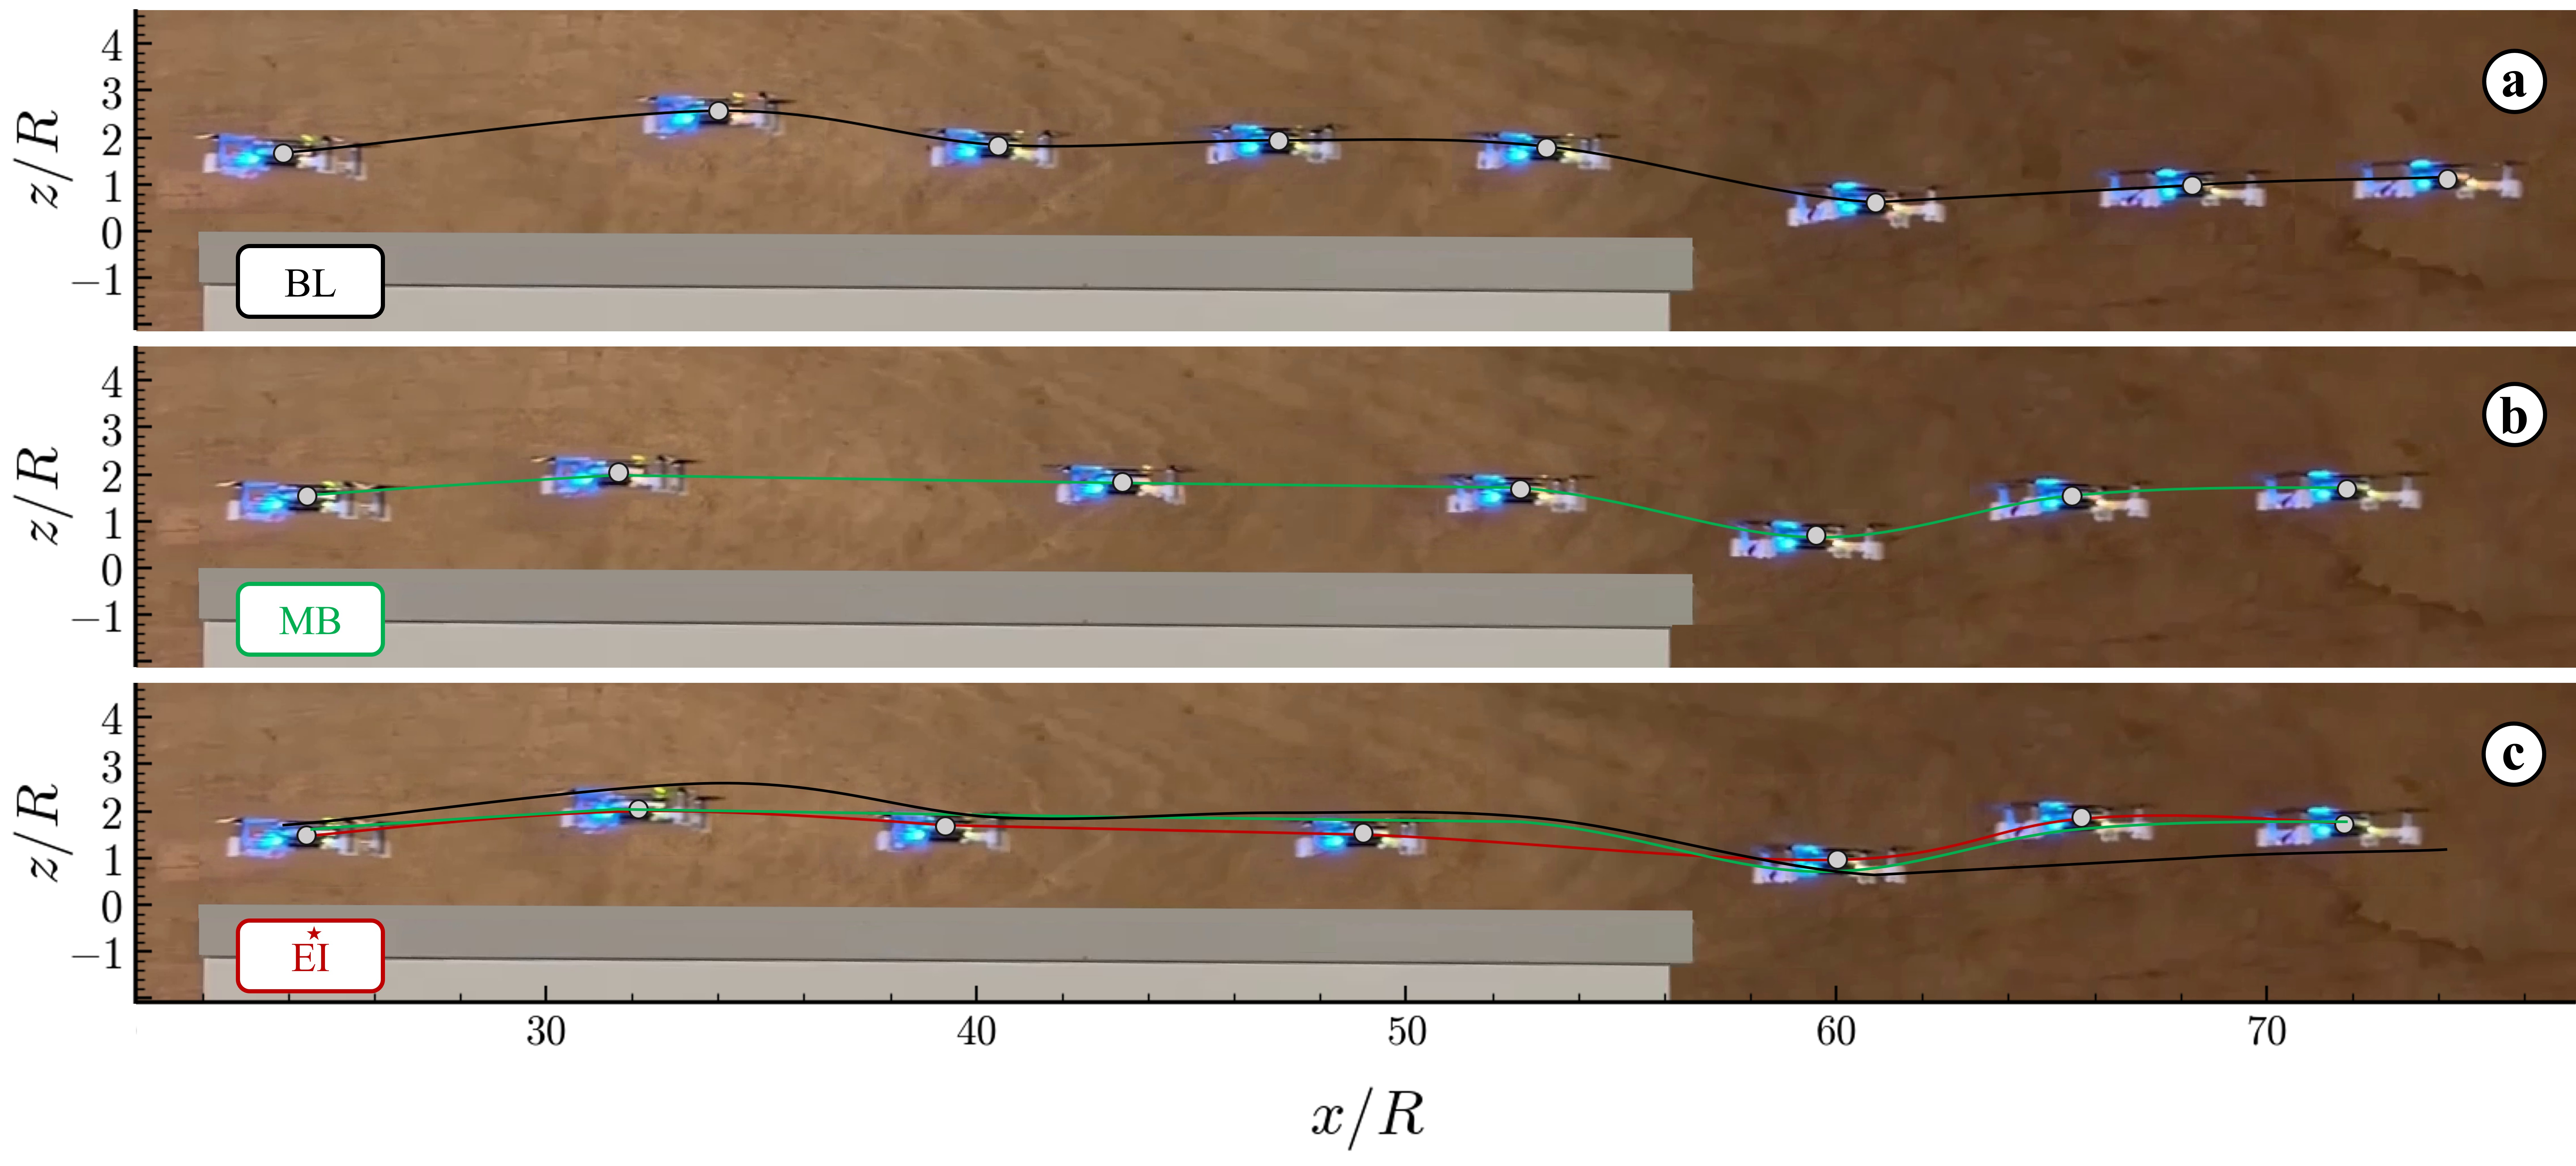
\includegraphics[width=\textwidth]{Results/Real_comparison.jpg}
\caption{Video-frame comparison of representative nominal-condition flights: (a) baseline policy $\pi_{\mathrm{BL}}$, (b) model-based policy $\pi_{\mathrm{MB}}$, and (c) best Expected-Improvement policy $\pi_{\mathrm{EI}}^{\star}$. The overlaid curves trace the measured vehicle path.}
\label{fig:real-comparison}
\end{figure*}

\subsection{Generalization Across Operating Conditions}
\label{sec:results-generalization}

Up to this point, the reward-transfer surrogate has been calibrated at the single nominal operating condition $(z^\ast/R,\,v_x^\ast/v_h)=(1.5,0.079)$. At this condition, the model-based policy produced a clear improvement over the baseline policy, and only a few additional physical evaluations were required for the GP discrepancy $\delta$ to capture part of the residual mismatch between the DT and physical rewards. Expected Improvement could consequently identify a policy with substantially better physical performance even though its DT reward was only marginally higher than that of $\pi_{\mathrm{MB}}$. The final campaign block investigates whether this policy correction remains useful when both the desired clearance and the forward velocity are changed.

Two additional operating conditions are considered: a low-speed, larger-clearance crossing at $(z^\ast/R,\,v_x^\ast/v_h)=(2.5,0.045)$ and a higher-speed, small-clearance crossing at $(1,0.113)$. The trajectory comparisons are reported in Fig.~\ref{fig:generalization-trajectories}. At each condition, the built-in PID controller executes the condition-specific baseline policy $\pi_{\mathrm{BL}}$, while a new model-based policy is computed using the same frozen parameter vector $\widehat{\boldsymbol{\theta}}_p$ identified at the end of the information phase. The nominal best correction is then transferred by applying the same three coefficients $\mathbf a=[a_A,a_B,a_C]^\top$ relative to the condition-specific model-based policy. This scaling preserves the learned correction structure without imposing the nominal reference correction as a fixed altitude offset.

In both operating conditions, the condition-specific model-based policy markedly improves tracking relative to the corresponding baseline policy. At $(z^\ast/R,\,v_x^\ast/v_h)=(2.5,0.045)$, the transferred policy provides a further, albeit modest, improvement. At the higher-speed, small-clearance condition $(1,0.113)$, however, its physical reward is slightly lower than that of the model-based policy. This loss is important: the transferred correction was learned from discrepancies measured only at the nominal condition $(1.5,0.079)$, whereas the relative importance of the unmodeled transients changes with velocity, clearance, and the magnitude of the model-based action. Transfer therefore provides an informed initialization, but it does not replace condition-specific learning when the operating condition moves away from the region represented in the reward-transfer surrogate dataset.

\begin{figure}[t]
\centering
\resultfigure{Results/stage_6_generalization_trajectory_comparison.pdf}
\caption{Generalization at (a) $(z^\ast/R,\,v_x^\ast/v_h)=(2.5,0.045)$ and (b) $(1,0.113)$: PID, local model-based, transferred RT, and condition-specific EI policies.}
\label{fig:generalization-trajectories}
\end{figure}

A direct comparison of rewards across these missions requires the different baseline difficulty to be removed. The DT and physical quantities are therefore normalized independently by their condition-specific baseline-policy values according to Eq.~\eqref{eq:normalized-score}. The DT and physical scores are denoted by $\mathcal S_{\circ}$ and $\mathcal S_{\bullet}$, respectively. By construction, $\mathcal S_e=0$ for the corresponding baseline policy and a larger value indicates a greater reduction of the tracking cost. This normalization places missions with different velocities and clearances on the same improvement scale and defines the normalized reward-transfer surrogate used across operating conditions.

In this more general formulation, the GP discrepancy depends on both the policy and the operating condition,
\begin{equation}
 \widehat{\mathcal S}_{\bullet}=
 \widehat{\mathcal S}_{\bullet,\mathrm{aff}}(\mathcal S_{\circ})+
 \widehat{\delta}\!\left(\mathbf a,z^\ast/R,v_x^\ast/v_h\right).
 \label{eq:generalized-surrogate}
\end{equation}
The vector $\mathbf a$ contains the three coefficients that modify the condition-specific model-based policy, while $(z^\ast/R,\,v_x^\ast/v_h)$ identifies the operating condition. Additional experiments distributed over the domain of interest would therefore train the normalized reward-transfer surrogate to propose a condition-specific correction instead of reproducing the same transferred policy everywhere. The present experiments provide an initial demonstration of this extension rather than a complete mapping of the velocity-clearance domain.

The normalized physical score is compared with its DT counterpart in Fig.~\ref{fig:generalization-reward}. Black markers correspond to $(z^\ast/R,\,v_x^\ast/v_h)=(1.5,0.079)$, orange markers to $(2.5,0.045)$, and purple markers to $(1,0.113)$. The transferred-policy diamond improves slightly on the model-based-policy square at the low-speed, larger-clearance condition. At the higher-speed, small-clearance condition, the ordering is reversed and the transferred policy performs slightly worse than $\pi_{\mathrm{MB}}$. A correction calibrated at one operating condition therefore cannot be assumed to retain the same ranking elsewhere, which motivates extending the surrogate across the operating domain rather than relying on direct policy transfer alone.

\begin{figure}[t]
\centering
\resultfigure{Results/stage_6_PID_normalized_reward_generalization.pdf}
\caption{Normalized reward-transfer surrogate across the nominal and two additional operating conditions.}
\label{fig:generalization-reward}
\end{figure}

The higher-speed, small-clearance condition is therefore used to demonstrate how the normalized reward-transfer surrogate can be extended locally. Two EI-guided physical evaluations are added at $(z^\ast/R,\,v_x^\ast/v_h)=(1,0.113)$. The first explores an uncertain policy direction and performs poorly, yielding approximately $\mathcal S_{\bullet}=0.57$, as indicated by the small purple marker in Fig.~\ref{fig:generalization-reward}. Once this observation updates the condition-aware GP discrepancy, the second evaluation reaches a new condition-specific best of approximately $\mathcal S_{\bullet}=0.83$, marked by the purple star, and exceeds the corresponding model-based policy. Its policy and physical trajectory are included in Fig.~\ref{fig:generalization-trajectories}(b). Unlike the nominal transferred correction, this policy remains closer to $\pi_{\mathrm{MB}}$, suggesting that the model-based policy was already near a favorable local optimum at the smaller clearance and higher velocity.

Only two condition-specific EI iterations are used here, so the result is interpreted as a proof-of-concept local extension of the RT workflow rather than as convergence of a general surrogate. At a new operating condition, the local DT first supplies a model-based policy that already improves substantially over the baseline policy. When direct transfer fails to improve that policy, a small number of physical interactions can reveal how the GP discrepancy has changed and redirect the search toward a better condition-specific solution. Repeating this process over the velocity-clearance domain would progressively calibrate $\widehat{\delta}(\mathbf a,z^\ast/R,v_x^\ast/v_h)$ and enable the generation of policies tailored to the requested operating condition while retaining the model-based policy as the safe and data-efficient reference.

\section{Conclusions and Outlook}
\label{sec:conclusion}

This work demonstrated Reinforcement Twinning for predictive trajectory control of a micro aerial vehicle crossing a finite obstacle in ground effect. The information phase provided evidence that the designed experiments added more than visual diversity: the cumulative smallest Fisher eigenvalue grew much faster than for repeated baseline experiments, and restricting the design from the broad domain to the near-wall domain restored information gain as the former began to saturate. Although the identified model parameters remained correlated, the resulting ground-effect function was well constrained over the control-relevant clearance range. Parameter decorrelation was therefore not treated as the objective by itself; the relevant outcome was the improved identification of the weakest observable parameter direction and of the aerodynamic correction used by the controller.

Model-based optimization remained the backbone of the framework. The identified DT generated an anticipatory model-based policy that improved tracking without replacing the onboard feedback controller and while satisfying the adopted virtual safety constraints. The remaining replay error then motivated the performance phase rather than invalidating the DT. Fractional and Sobol policies calibrated the reward-transfer surrogate, while Expected Improvement directed subsequent physical experiments toward uncertain and potentially better policies. With few additional interactions, the resulting $\pi_{\mathrm{EI}}^{\star}$ outperformed the model-based policy by compensating for response features that the low-order static model could not rank accurately. In this way, the DT restricted the search to a screened, high-performing neighborhood, and physical rewards were used specifically to learn the GP discrepancy within that neighborhood.

The off-nominal experiments clarified both the potential and the present limits of generalization. Directly transferring the nominal correction produced a modest gain at one operating condition but slightly underperformed the corresponding model-based policy at the other. After two condition-specific EI evaluations, the normalized reward-transfer surrogate identified an improved local policy. This result supports the data efficiency of local refinement, but it does not establish a surrogate that is converged over a continuous velocity-clearance domain.

The conclusions are therefore limited to the tested envelope. The ground-effect model represents an unsteady rotor-surface interaction with a static two-parameter law and cannot reproduce every transient feature. The physical experiments were constrained to $z/R\geq0.5$, so the results do not support extrapolation toward contact, and generalization was examined at only two additional operating conditions. Future work should extend the campaign across a denser velocity-clearance domain, account explicitly for repeated-measurement uncertainty in the reward-transfer surrogate, and investigate richer unsteady aerodynamic models, moving landing surfaces, and onboard or real-time policy adaptation. Within the present limits, the campaign shows how RT can combine interpretable physics, virtual safety screening, and a targeted data-driven correction to improve control performance without requiring unconstrained model-free exploration.

\section*{Acknowledgment}
The authors gratefully acknowledge the technical support of the von Karman Institute for Fluid Dynamics.

\bibliographystyle{IEEEtran}
\bibliography{references}

\end{document}





